% ---------------------------------------------------------------
% Chapter 4: imported 12 Sep 2026 from the subject-choice Overleaf
% project ("The productivity and diversity costs of constraints to
% subject choice", Advani, Drayton and Phelan). The text is the
% paper's, unchanged except for mechanics: article -> chapter
% structure, \input paths moved to tables/ch4/ and figures/ch4/,
% (\cite{...}) -> \citep / textual \cite -> \citet for the thesis's
% natbib setup, mojibake repaired (pound signs, dashes), and two
% dangling \ref targets pointed at the labels that exist
% (tab:earnings -> tab:main; sec:simulation_details ->
% sec:Appendix_Simulation). The paper's own \redbf{XX} placeholders
% are deliberately left in place and render in red.
% ---------------------------------------------------------------
\chapter{The Productivity and Diversity Costs of Constraints to Subject Choice}
\label{ch:paper3}
\resetcounterformats

\begin{center}
  \textit{Arun Advani, Elaine Drayton and Damian Phelan%
    \thanks{Arun Advani: University of Warwick, CenTax, and Institute for
      Fiscal Studies. Elaine Drayton: Institute for Fiscal Studies. Damian
      Phelan: University College London and Institute for Fiscal Studies.
      The authors thank Jack Britton, Laura van der Erve, Christine
      Farquharson, Ross Warwick \redbf{ANYONE ELSE?} and seminar
      participants at the IFS and CEPEO \redbf{ANYWHERE ELSE}. This
      research was supported by the Economic and Social Research Council
      (ES/W010224/1).}}
\end{center}

\begin{chapterabstract}
School and university subject choices are an important determinant of career pathway and hence lifetime wages. We show that access to high return subjects varies systematically across regions and demographic groups of school students in England. Using within-school variation in access, consistent with the arrival or departure of a subject teacher within a school, we show this has a large causal impact on subject studied at university. Using linked education and employment data, we document the cost in terms of lifetime income of not having access to certain subjects at school; the cost estimates rest mainly on precisely estimated effects on university attendance and degree choice combined with published lifetime returns by degree subject, while the direct age-28 earnings estimate points the same way but is less precise. Because availability is lowest outside London and the South East, expanding it would also shift the intake of high-return degrees towards under-represented regions. We estimate that the fiscal return to additional teachers in high return subjects exceeds the cost of recruiting, training and employing them under both of our costing constructions.
\end{chapterabstract}

%%%%%%%%%%%%%%%%%%%%%%%%%%%%%%%%
\section{Introduction}
\label{sec:Introduction}
%%%%%%%%%%%%%%%%%%%%%%%%%%%%%%%%
% --- Paragraph 1: The misallocation problem ---

Field of study is one of the largest determinants of lifetime earnings. The gap between the highest- and lowest-return university subjects rivals the entire college wage premium \citep{altonji2016handbook}, and causal estimates confirm that much of this gap reflects the effect of the field itself, not selection \citep{kirkeboen2016field,bleemer2022college}. Yet access to high-return fields is not equally distributed: who gets to choose depends on institutional constraints that vary across schools, regions, and demographic groups \citep[e.g.][]{goodman2019math}. Such constraints cause human capital misallocation that can have large aggregate growth costs \citep{hsieh2019allocation}, but micro-level evidence on which specific constraints matter and what it costs to remove them is scarce. Existing causal estimates of field-of-study returns identify effects at competitive margins, such as admission cutoffs and GPA thresholds, rather than at the extensive margin of whether the option to choose exists at all.

% --- Paragraph 2: This paper ---

We study the causal effect of taking economics at A-level -- the main upper-secondary qualification in England -- on university subject choice and lifetime earnings. Our instrument is within-school, across-cohort variation in whether a school offers A-level economics, consistent with the arrival or departure of a suitably qualified teacher. We do not observe teachers directly: provision is inferred from exam sittings, and we present evidence below that the within-school changes we exploit behave like supply shocks. Using population-level linked administrative data that follow students from age 11 through university and into the labour market, we show that taking A-level economics substantially increases the probability of studying economics at university, and we find evidence of substantial earnings gains for the students whose choices are shifted. We estimate the marginal value of public funds (MVPF) of hiring additional economics teachers and find that the policy more than pays for itself.

% --- Paragraphs 3-4: Setting and why it matters beyond the UK ---

%Note to self: this para could be tighter. Still has a lot about university, which we don't nec want so up front
England provides an unusually clean setting for studying supply-side constraints on subject choice. At age 16, students select three or four subjects to study at A-level, and these choices largely determine which degree they can pursue at university. A-level economics is the principal gateway to an economics degree: students who take it are 27--29 percentage points more likely, in raw and covariate-adjusted terms, to study economics at university than those who do not.\footnote{In the pooled 2002--2008 sample, 29.5\% of A-level economics takers study economics at university, against 0.9\% of non-takers: a raw gap of 28.6 percentage points, or 27.3 controlling for attainment and demographics.} But fewer than half of schools offer A-level economics, and whether a school does so depends primarily on whether it employs a teacher qualified to teach the subject. There is no centralised competitive selection for A-level economics places: schools may set general sixth-form entry requirements, but conditional on entering the sixth form the subject is not rationed, so this is a binary supply constraint rather than a rationing problem. Either the school has an economics teacher and offers the subject, or it does not.

The principle that supply-side constraints on high-return human capital matter is general; the English institutional setting provides three features that make it possible to measure the effect cleanly. First, students typically remain in the same secondary school, or move to its linked school, from age 11 to 18, so school choice at age 11 is unlikely to reflect anticipated A-level economics availability years later. Second, whether a school offers economics varies across cohorts within the same school, with roughly one-third of schools switching between offering and not offering economics over our sample period, generating within-school variation that is plausibly driven by staffing changes rather than by shifts in student characteristics. Third, the Longitudinal Education Outcomes (LEO) dataset links the universe of school records, university enrolment, and tax-based earnings data, allowing us to trace the consequences of school-level subject access through to adult labour market outcomes at population scale.

% --- Paragraphs 5-6: Data and identification ---

Our sample comprises all students who completed GCSEs (nationally graded exams at age 16) in England between 2002 and 2008 and continued to A-level study, for whom we observe earnings through to age 28. % Damien: I think we should just switch to 2009 consistently. Doesn't make sense to do the descriptives on a different sample here I think
% Our sample comprises all students who completed GCSEs (nationally graded exams at age 16) in England between 2002 and 2013. For the earnings analysis, we restrict to the 2002--2009 GCSE cohorts, for whom we observe earnings through to age 28.
The instrument is an indicator for whether a student's school offered A-level economics to their cohort. We include school fixed effects, to absorb all time-invariant differences between schools -- including long-run attainment levels, socioeconomic composition, and resource availability -- so that identification comes solely from within-school changes in whether the subject is offered. Cohort fixed effects and rich individual-level controls for prior attainment, demographics, and socioeconomic background address time-varying confounders.

% We assess the plausibility of the exclusion restriction through several checks: balance tests confirming that within-school changes in economics availability do not predict pre-treatment outcomes such as GCSE scores; placebo regressions on students who do not study economics at university; specifications including school-specific linear time trends; and models with region-by-year fixed effects. \redbf{Across all checks, we find no evidence that availability changes are systematically correlated with pre-treatment characteristics or outcomes for non-compliers.}

% --- Paragraphs 7-9: Key results ---

% Result 1: Access
We report three sets of results. First, we document that access to A-level economics is unequally distributed along every dimension we examine -- sex, ethnicity, socioeconomic status, and geography. Differences in whether schools offer the subject, rather than differences in student preferences or attainment, explain 36\% of the regional take-up gap -- the largest gap we observe, and the share is stable across cohorts -- and between 6\% and 75\% of the take-up gaps across demographic groups. The 75\% share applies to the gap by free school meal status, which is small (0.4 percentage points) but almost entirely a matter of access. Students eligible for free school meals (FSM), a standard administrative marker of low socio-economic family background, are around 3 percentage points less likely to attend a school that offers economics than their non-FSM peers. Students in London and the South East of England are up to 35 percentage points more likely to have access than students in the Midlands, North East, or South West.\footnote{From the full regional breakdown of 2011 access rates: London 82.0\%, North East 46.8\%, South West 55.8\%, East Midlands 56.6\%, West Midlands 60.3\%. Table~\ref{tab:access_takeup} reports the two-way London/South East split.} %NTS: maybe regional info is too much detail for intro?

% Result 2: Impact
Second, we estimate the causal effect of taking A-level economics on earnings. The first stage is strong: within-school availability of A-level economics increases the probability of taking the subject by 5.7 percentage points ($F = 843$). Students induced to take A-level economics are 15.2 percentage points more likely to study economics at university, confirming the gateway role documented in our descriptive analysis. The IV estimate implies that taking A-level economics raises earnings at age 28 by around 14\%, though this estimate is significant only at the 10\% level, with a 95\% confidence interval running from roughly zero to 27 log points. Combining our estimates with published estimates of lifetime returns by degree subject \citep{britton2026lifetime}, the implied lifetime gain is approximately \pounds 190,000 in present value (gross) and \pounds 90,000 net of tax and student loan repayments. These lifetime figures rest mainly on the two precisely estimated education margins --- university attendance and degree choice --- combined with the published returns, rather than on the age-28 earnings estimate itself.
%The magnitude of the local average treatment effect reflects the characteristics of the complier group: students who take A-level economics when it is offered but would not otherwise, for whom the returns are likely to be particularly high. %% BUT MAYBE NOT ACTUALLY, BECAUSE ALTHOUGH THOSE WHO CHOOSE TO TAKE POTENTIALLY HAVE A HIGHER RETURN TO IT THAN THOSE WHO DON'T, CONDITIONAL ON BEING OFFERED, THE WHOLE POINT IS THAT IN OUR CASE. ACTUALLY, OTHER WAY AROUND - WE SHOULD EXPECT HIGHER RETURNS THAN OTHER CONTEXTS, BECAUSE IT ISN'T RATIONING AT THE MARGIN. SOME VERY INFRAMARGINAL PEOPLE WITH POTENTIALLY INCREDIBLY HIGH RETURNS ARE CURRENTLY RULED OUT. WAIT TIL NUMBERS ARE IN, THEN REWRITE ACCORDINGLY
The implied lifetime gain is constructed mainly from the shift into economics degrees, which carry among the highest lifetime returns of any subject: the 15.2 percentage point increase in economics degree take-up among compliers, combined with a net lifetime return to an economics degree of around \pounds 560,000 \citep{britton2026lifetime}, accounts for roughly 85\% of the calculation. The age-28 evidence points to broader channels --- the observed earnings gains sit mainly with compliers who do not change degree subject --- so we also report an alternative construction based on persistence of the age-28 premium, which gives a similar order of magnitude.

% Result 3: Policy
Third, we compute the return to expanding access. If all schools offered A-level economics, our estimates imply an additional 4,000 students per cohort would take A-level economics, of whom approximately 630 would go on to study economics at university, shifting the composition of the intake towards regions outside London and the South East, with smaller movements by sex and socioeconomic background. We estimate that the MVPF of hiring an additional economics teacher is infinite: the fiscal returns from higher lifetime tax revenue exceed the salary and training costs of the teacher, so that the policy pays for itself; the conclusion survives even if the estimated returns are overstated by two-thirds. Because the supply constraint binds most tightly outside London and the South East, removing it improves allocative efficiency while shifting the intake of economics degrees towards under-represented regions. The compositional gains by sex and socioeconomic background are small, and the equity case rests on the access evidence rather than on any demonstrated difference in returns across groups.

% --- Paragraphs 10-12: Contribution relative to literature ---

% Lit 1 (returns to field of study -- extensive margin):
Causal estimates from admission lotteries and scoring cutoffs have established that field of study is a major determinant of earnings --- comparable in magnitude to the college wage premium itself --- and that much of this variation reflects the effect of the field, not selection \citep{kirkeboen2016field,bleemer2022college,hastings2013cutoffs}. For the UK, \citet{britton2020degrees} document large variation in lifetime returns across degree subjects using the same administrative data we use. Closest to our margin, \citet{dahl2023highschool} estimate long-run earnings effects of upper-secondary fields of study in Sweden; we differ in studying whether the field is available at all. All of these estimates are identified at the selection margin: who gains a place when competition is binding. We estimate the return at the extensive margin --- what happens when the option to study a high-return subject does not exist. This distinction matters for policy. Expanding access at a competitive cutoff displaces other applicants; expanding access at the extensive margin does not. The complier population is also different: rather than students at a scoring threshold, our compliers are students who would study economics if it were available but currently cannot.

% Lit 2 (misallocation -- micro evidence on a removable barrier):
A growing body of work argues that barriers preventing talented individuals from entering high-return occupations impose large aggregate costs. \citet{hsieh2019allocation} attribute 20--40 \% of US output growth between 1960 and 2010 to improved allocation of talent across occupations, using a calibrated Roy model applied to observed changes in the occupational distribution. Their framework implies that removing specific barriers would generate measurable gains, but does not isolate any individual barrier or estimate the cost of removing it. We provide the type of micro evidence their framework calls for: a concrete, causally identified barrier (the absence of a subject teacher), an estimate of the earnings consequences of removing it, and a cost-benefit calculation showing the barrier can be eliminated at negative net fiscal cost. We compute the marginal value of public funds \citep{hendren2020mvpf} for expanding teacher supply, connecting the misallocation literature to the welfare-evaluation framework that has become standard in applied public economics.

% Lit 3 (supply-side constraints vs. demand-side interventions):
Research on underrepresentation in economics and other high-return fields has focused predominantly on demand-side interventions: exposing students to role models \citep{porter2020rolemodel}, redesigning introductory courses \citep{bayer2020you}, providing information about career prospects \citep{avilova2018can}, and mentoring \citep{blau2010can}. These interventions implicitly assume that students have the option to study economics and the question is whether they choose to. We show that for a substantial fraction of students the constraint is more basic: the subject is not available at their school. Our preference-constraint decomposition indicates that availability alone accounts for 36\% of the regional gap in A-level economics take-up, and between 6\% and 75\% of the gaps across demographic groups, before preferences enter. Because schools serving disadvantaged students are least likely to offer economics, supply-side constraints compound existing inequalities. The causal estimates show that relaxing these constraints shifts students into high-return educational and career paths, and the cost-benefit calculation shows that the fiscal return exceeds the cost of additional teachers. Supply-side interventions are therefore a necessary complement to the demand-side measures that have dominated the policy discussion.

% --- Paragraph 13: Roadmap ---

The paper proceeds as follows. Section~\ref{sec:Data} describes the data and institutional context. Section~\ref{sec:Access} documents the unequal distribution of access to A-level economics and decomposes take-up gaps into preference-driven and constraint-driven components. Section~\ref{sec:Impact} presents the empirical framework and estimates the causal effect of A-level economics on degree choice, earnings, and lifetime income. Section~\ref{sec:Policy} computes the MVPF of expanding teacher supply and presents a counterfactual exercise on universal access. Section~\ref{sec:Conclusion} concludes.


%%%%%%%%%%%%%%%%%%%%%%%%%%%%%%%%
\section{Data and Institutional Context}
\label{sec:Data}
%%%%%%%%%%%%%%%%%%%%%%%%%%%%%%%%

Students in England follow a structured educational pathway with two critical transition points relevant to this paper. At age 14--16, students study for the General Certificate of Secondary Education (GCSE), a set of nationally graded examinations covering a broad curriculum. GCSE results determine eligibility for further study and serve as the main measure of prior attainment in our analysis. At age 16, students who continue to upper-secondary education select three or four subjects to study at Advanced Level (A-level) over two years. A-level choices are consequential: they largely determine which degree subjects a student can pursue at university. A student who does not take A-level economics, for instance, will find it difficult to gain admission to an economics degree at most universities. Additionally, since economics is almost never taught at any earlier stage at school, students who do not study it at A-level are unlikely to be aware of it as a subject \citep{smith2025discoverecon}. Whether a school offers A-level economics depends primarily on whether it employs a suitably qualified teacher: a supply constraint we exploit for identification.

Most students --- 71\% --- stay in the same secondary school, or move to its linked school, from age 11 to 18, though at the end of GCSE (age 16) some transfer to a different institution for A-levels, either by choice or because their school does not offer post-16 education. We discuss the implications of school-changing for identification in Section~\ref{sec:Impact}.

We use the Longitudinal Education Outcomes (LEO) dataset, which links three administrative sources covering the universe of state and private school students in England. The National Pupil Database (NPD) provides individual-level demographic characteristics (sex, ethnicity, free school meal eligibility), school identifiers, and attainment at each Key Stage, including GCSE and A-level results. The Higher Education Statistics Agency (HESA) records provide information on university attendance, institution, and degree subject. His Majesty's Revenue and Customs (HMRC) tax records provide annual earnings from employment and self-employment. The linked dataset allows us to follow each student from their GCSE results at age 16 through A-level and university choices and into the labour market.

% Our full sample comprises all students who completed GCSEs in England between 2002 and 2009 \redbf{WE SHOULD STICK TO SAME SAMPLE THROUGHOUT}. We use this sample for the descriptive analysis of access and take-up in Section~\ref{sec:Access}. For the earnings analysis in Section~\ref{sec:Impact},
We observe school-level provision of A-level economics for the wider window of GCSE cohorts 2002--2013, which the descriptive figures draw on. We restrict the estimation sample to the 2002--2008 GCSE cohorts, for whom we observe earnings at age 28 (the latest year in our earnings data is 2021). Identification in Section~\ref{sec:Impact} comes from within-school changes in availability, to which always-offer and never-offer schools contribute nothing once school fixed effects are included; the estimation samples are therefore restricted to students in switcher schools, with offer behaviour classified over the full sample window. The analysis population is students who continue to Key Stage 5 (A-level study): students who leave education at 16 are not at risk of taking any A-level, so the access and take-up rates in Section~\ref{sec:Access} and the estimation samples below are all defined on this population. Continuation could in principle itself respond to availability, which would make entry into the population endogenous; the balance tests and the KS4 intake event study in Section~\ref{sec:Impact} show no compositional response to within-school availability changes, and within the population, sample inclusion is unrelated to the instrument, as reported below. Of the 1,449,714 student records in the 2002--2008 cohorts, 1,409,352 have university outcomes observed and 1,231,580 have positive earnings at age 28. The university-outcome regressions use the 417,849 switcher-school students among the former with all controls observed --- Key Stage~2 attainment, which the controls include, is missing for around six per cent of students --- and the earnings regressions the 368,260 among the latter; the levels specification, which retains students with zero earnings, uses 406,352. Inclusion in the estimation sample is unrelated to the instrument: regressing an indicator for inclusion in the earnings sample on availability, with school and cohort fixed effects, gives a coefficient of $-0.0004$ (standard error $0.0015$). We focus on age-28 earnings as the primary outcome because it is the latest age observed for all cohorts, and combine these estimates with published estimates of lifetime returns by degree subject \citep{britton2026lifetime} to assess lifetime effects.

We measure A-level economics availability using a school-cohort indicator equal to one if at least two students in the school-year group sat the A-level economics examination.\footnote{We do not observe subject offerings directly, so we infer availability from take-up. Availability is measured from the complete exam records, before any sample restriction. We require at least two students rather than one because a single student taking economics may be doing so at a neighbouring school or by studying at home rather than at their own. Such actions are unusual, and where they occur would represent a substantially higher cost of access. Appendix Table~\ref{tab:threshold_robustness} shows the main results using thresholds of one to five students. The instrument is strong and the IV estimate positive at every threshold, and the estimates rise with the threshold, from 0.135 at two students to 0.256 at five. We read this range as genuine uncertainty about the size of the estimate across codings; the baseline threshold of two gives the smallest point estimate, so the headline numbers are the most conservative of the set. Because availability is inferred from take-up, part of the first-stage association is mechanical --- cohorts coded as non-offering have at most one taker by construction --- though the reduced-form effects on earnings and degrees are not mechanically linked to the coding. The seven-percentage-point jump in take-up at a switch, ten to fifteen students in a typical sixth form, is difficult to rationalise as smooth demand variation around a two-student threshold, supporting the supply interpretation.} This is the instrument in our IV design. Because provision is inferred from exam sittings rather than observed directly, part of the first-stage association is mechanical, and we treat the reduced-form effects on earnings and degree choice --- which are not mechanically linked to the coding --- as the cleaner objects; the footnote above and Appendix Table~\ref{tab:threshold_robustness} set out the consequences of the coding choice. Across our sample, the share of schools offering A-level economics by this measure rises gradually from 38\% to 42\% over the estimation window, and reaches 46\% by 2011 (Appendix Figure~\ref{fig:time_series}). Around one-third of schools switch between offering and not offering economics (or vice versa) at some point our sample period, generating the within-school variation that drives identification (see also Figure~\ref{fig:sequence}).

% Table: Summary statistics by school offer type (Chapter 4)
\begin{table}[htbp]
\centering
\caption{Summary statistics by school economics offer behaviour}
\label{tab:summary_stats}
\begin{tabular}{l cccc}
\toprule
                              & All        & Switcher   & Always     & Never      \\
                              &            & offer      & offer      & offer      \\
\midrule
\multicolumn{5}{c}{\textbf{Panel A: Student characteristics}} \\
\midrule
N students                    & 221,118         & 60,762         & 119,665         & 40,691         \\
\% female                     & 54.7         & 57.2         & 52.4         & 57.5         \\
\addlinespace
\% White British              & 71.8         & 73.2         & 68.6         & 79.3         \\
\% Indian                     & 3.6         & 2.7         & 4.6         & 2.3         \\
\% Pakistani/Bangladeshi      & 4.3        & 4.2         & 4.2         & 4.8         \\
\% Black African/Caribbean    & 4.1         & 4.4         & 4.5         & 2.6         \\
\% Chinese                    & 0.8         & 0.7         & 0.9         & 0.5         \\
\% Other ethnicity            & 10.6         & 11.0         & 11.3         & 7.8         \\
\addlinespace
\% FSM eligible               & 9.0         & 7.1         & 5.6         & 7.5         \\
Mean std.\ GCSE score         & 0.63         & 0.60         & 0.64         & 0.63         \\
\midrule
\multicolumn{5}{c}{\textbf{Panel B: Subject choices and outcomes}} \\
\midrule
\% taking A-level economics   & 6.8         & 4.2         & 10.4         & 0.1         \\
\% attending university       & 81.5         & 80.5         & 83.5         & 77.4         \\
\% studying economics at UG   & 2.6         & 2.0         & 3.5         & 0.9         \\
\addlinespace
Mean log earnings at 28       & 10.24         & 10.22         & 10.28         & 10.17         \\
N (earnings sample)           & 1,409,352         & 444,936         & 651,372         & 313,026         \\
\bottomrule
\end{tabular}
\begin{minipage}{\textwidth}
\smallskip
\footnotesize
\textit{Notes:} The table reports means for the 2011 GCSE cohort. School offer behaviour is defined over the full sample period: ``Always offer'' schools offer A-level economics in every cohort; ``Never offer'' schools never offer it; ``Switcher'' schools offer it in some cohorts but not others. A school is defined as offering A-level economics if at least two students in the school-year group sit the exam. The earnings sample is restricted to the 2002--2008 GCSE cohorts, for whom earnings at age 28 are observed. Standardised GCSE score has mean zero and unit variance in the full population.
\end{minipage}
\end{table}


Table~\ref{tab:summary_stats} presents summary statistics for the 2011 GCSE cohort, the cohort used for the descriptive access analysis, with the final panel describing the 2002--2008 estimation cohorts; each is shown overall and separately for three categories of schools defined by their offering pattern across cohorts: always-offer schools, which provide A-level economics in every year they appear in our data; never-offer schools, which never do; and switcher schools, which change status at least once. The first column covers all schools. The remaining columns reveal systematic differences across school types that motivate our identification strategy. Always-offer schools have higher average GCSE attainment, lower shares of students eligible for free school meals, and higher shares of students from ethnic groups that disproportionately study economics at university. Never-offer schools are the mirror image. Switcher schools---the source of our identifying variation---lie between the two on most observable dimensions; on attainment and single-sex composition they resemble never-offer schools. These differences underscore the importance of school fixed effects, which absorb all time-invariant differences between schools and ensure that identification comes solely from within-school changes in availability. We discuss the characteristics of switcher schools further in Section~\ref{sec:Impact}, where we present the empirical framework.


%%%%%%%%%%%%%%%%%%%%%%%%%%%%%%%%
\section{Who gets to study economics?}
\label{sec:Access}
%%%%%%%%%%%%%%%%%%%%%%%%%%%%%%%%

% --- Paragraph 1: Supply constraints matter ---

Whether a student can take A-level economics depends largely on where they go to school. Students in London and the South East are 15.3 percentage points more likely to attend a school that offers economics than students in the rest of England: a gap too large to reflect differences in student aptitude or interest, and one that instead reflects which schools employ an economics teacher. Across England in 2011, only 46\% of schools offered A-level economics (Appendix Figure~\ref{fig:time_series}). Students in the remaining schools cannot choose a subject with among the highest returns of any A-level, both directly and through its role as the principal pathway to an economics degree.

% --- Paragraph 2: Broader access patterns (gender, FSM, region) ---

Table~\ref{tab:access_takeup} documents access rates, take-up conditional on access, and unconditional take-up for the 2011 GCSE cohort, broken down by sex, socioeconomic status, region, and ethnicity. The regional gap is the starkest dimension, but it is not the only one. Students eligible for free school meals are 3.5 percentage points less likely to attend a school offering economics than their non-FSM peers. Women have lower access than men (66.0\% versus 70.1\%), but are also less likely to take the subject conditional on access (5.6\% versus 15.0\%), indicating the role of preferences alongside constraints. Appendix Table~\ref{tab:school_type} shows the same pattern by school type: where economics is offered, girls in single-sex schools take it at around twice the rate of girls in mixed schools. Indian and Chinese students have both higher access and conditional take-up than White students, while the reverse is true for Pakistani, Bangladeshi and Black students, mirroring the broader socioeconomic patterns for these groups.

% Table: Access to and take-up of A-level economics by demographic group (Chapter 4)
\begin{table}[htbp]
\centering
\caption{Access to and take-up of A-level economics by demographic group, 2011 cohort}
\label{tab:access_takeup}
\begin{tabular}{l ccccc}
\toprule
                              & Access     & Take-up    & Take-up    & Gap from   & Share of   \\
                              & rate       & $|$ access & (uncondit.)& access     & gap from   \\
                              &            &            &            &            & access     \\
\midrule
\multicolumn{6}{c}{\textbf{Panel A: Sex}} \\
\midrule
Male                          & 70.1         & 15.0         & 10.5         &            &            \\
Female                        & 66.0         & 5.6         & 3.7         &            &            \\
Gap (M $-$ F)                 & 4.1         & 9.4         & 6.8         & 0.4         & 5.9         \\
\midrule
\multicolumn{6}{c}{\textbf{Panel B: Socioeconomic status}} \\
\midrule
Non-FSM                       & 68.4         & 9.9         & 6.8         &            &            \\
FSM                           & 64.9         & 9.8         & 6.4         &            &            \\
Gap                           & 3.5         & 0.1         & 0.4         & 0.3         & 75.0         \\
\midrule
\multicolumn{6}{c}{\textbf{Panel C: Region}} \\
\midrule
London/South East             & 77.8         & 12.3         & 9.6         &            &            \\
Rest of England               & 62.5         & 8.3         & 5.2         &            &            \\
Gap                           & 15.3         & 4.0         & 4.4         & 1.6         & 36.4         \\
\midrule
\multicolumn{6}{c}{\textbf{Panel D: Ethnicity}} \\
\midrule
White British                 & 65.3         & 8.2         & 5.4         &            &            \\
Indian                        & 78.9         & 20.2         & 16.0         &            &            \\
Pakistani/Bangladeshi         & 67.8         & 12.8         & 8.7         &            &            \\
Black African/Caribbean       & 77.9         & 14.0         & 11.0         &            &            \\
Chinese                       & 75.7         & 21.3         & 16.4         &            &            \\
\addlinespace
Gap: Indian $-$ White         &            &            & 10.6         & 1.9         & 17.9         \\
Gap: Pak./Bang. $-$ White.     &            &            & 3.3         & 0.3         & 9.1         \\
Gap: Black Afr./Car. $-$ White &            &            & 5.6         & 1.4         & 25.0         \\
Gap: Chinese $-$ White        &            &            & 11.0         & 1.5         & 13.6         \\
\bottomrule
\end{tabular}
\begin{minipage}{\textwidth}
\smallskip
\footnotesize
\textit{Notes:} Access rate is the share of students attending a school that offers A-level economics (defined as $\geq 2$ students sitting the exam in the school-cohort). Take-up $|$ access is the share taking A-level economics conditional on the school offering it. The take-up gap between groups $A$ and $B$ is decomposed as $p_A - p_B = \bar{c}(a_A - a_B) + \bar{a}(c_A - c_B)$, where $a$ denotes the access rate, $c$ denotes conditional take-up, and bars denote simple averages across the two groups. ``Gap from access'' reports the first term: the component of the take-up gap attributable to differential access, holding conditional take-up at the cross-group average. ``Share of gap from access'' divides this by the unconditional take-up gap. For ethnicity, gap directions are chosen so that a positive unconditional gap corresponds to the group listed first having higher take-up. Sample: 2011 GCSE cohort, $N = $ \redbf{XX}.
\end{minipage}
\end{table}


% --- Paragraph 3: Isn't just pre-existing differences ---
%IF WE GET TIGHT FOR SPACE, THIS IS A GOOD CANDIDATE FOR TIGHTENING, DON'T NEC HAVE TO GO THROUGH IT ALL

Table~\ref{tab:access_takeup} also helps distinguish the mechanism behind these gaps. For FSM students, take-up conditional on access is almost identical to that of their non-FSM peers, so their lower unconditional take-up reflects where they go to school rather than weaker demand for economics. For ethnic groups, by contrast, large differences in conditional take-up remain: Indian and Chinese students are substantially more likely to choose economics than White British students even where both have access, and Pakistani, Bangladeshi and Black African and Caribbean students also choose it at higher rates. This indicates that preferences and demand-side factors shape economics take-up alongside supply constraints. Appendix Table~\ref{tab:lpm_subgroup} reports regression counterparts of these patterns: the effect of availability on take-up estimated separately for each subgroup.

% \redbf{TO DISCUSS: HOW ARE WE IDENTIFYING A BINARY TREATMENT (OFFER) AND TWO FIXED EFFECTS FOR SCHOOL TYPE? I think we might only want offer * always, and offer * switcher. Currently the model is neither fully saturated, nor fully constrained, so the switcher fixed effect is picking up the difference in take up when economics isn't offered i.e. people studying it solo. ACTUALLY, DECIDED TO JUST MOVE FROM LPM TO ACCOUNTING DECOMP}

% --- Paragraph 4: Decomposition ---

How much of the overall gap in take-up is explained by supply constraints versus preferences? We decompose the unconditional take-up gap between any two groups into an access component and a preference component using the descriptive statistics in Table~\ref{tab:access_takeup}.\footnote{For groups $A$ and $B$ with access rates $a_A, a_B$ and conditional take-up rates $c_A,c_B$, the unconditional take-up gap decomposes as $p_A - p_B = \bar{c}(a_A - a_B) + \bar{a}(c_A - c_B)$, where $\bar{c}$ and $\bar{a}$ are simple averages across the two groups. The first term is the access component: the share of the gap attributable to differential availability, holding conditional take-up at the cross-group average. The second is the preference component: the share attributable to differential take-up conditional on access, holding access constant. This is an accounting identity, not a causal decomposition; the causal effect of access on take-up is estimated in Section~\ref{sec:Impact}.} The access component measures the mechanical contribution of differential availability: how much smaller the take-up gap would be if both groups had equal access. The preference component captures the residual: differences in take-up conditional on the subject being available, reflecting tastes, information, peer effects, and other demand-side factors.

The final two columns of Table~\ref{tab:access_takeup} report these components for each pairwise comparison. The regional gap is the clearest case: students in London and the South East have substantially higher access than students elsewhere, but conditional take-up rates differ more moderately (12.3\% versus 8.3\%), so that 36.4\% of the regional take-up gap is attributable to access alone. %This is the pattern the misallocation framework of \cite{hsieh2019allocation} predicts: latent demand exists where supply does not, and the resulting mismatch is wasteful. - REPHRASE AT SOME POINT, BUT BRING BACK THE HSIEH REF HERE

% --- Paragraph 5: Subgroup decomposition ---

The other panels of Table~\ref{tab:access_takeup} show three distinct patterns. For socioeconomic status, conditional take-up is essentially identical: where economics is offered, FSM and non-FSM students take it at almost the same rate (9.8\% against 9.9\%). The take-up gap between the two groups is therefore almost entirely a matter of access: the access component accounts for 75\% of it, though the gap itself is small, at 0.4 percentage points. For sex, the opposite holds. Women have somewhat lower access than men, but the far larger difference is in take-up where the subject is available (5.6\% against 15.0\%), so the access component explains only 5.9\% of the gap. Supply-side expansion is necessary but not sufficient for closing the gender gap; demand-side interventions matter too \citep{porter2020rolemodel,smith2025discoverecon}.

For ethnicity, the gaps run the other way: all four minority groups in the table have higher take-up than White British students. For Indian and Chinese students the preference component dominates --- these groups have strong demand that is largely met by supply, with access accounting for 17.9\% and 13.6\% of their take-up gaps. For Black African and Caribbean students a quarter of the gap (25.0\%) is attributable to access, and for Pakistani and Bangladeshi students 9.1\%. The contrast across groups reinforces the point that the constraint operates through school-level supply, not ethnicity itself.

Across all comparisons, the access component explains between 6\% and 75\% of the take-up gap. This range provides a transparent lower bound on the role of supply constraints: it takes no stand on the causal effect of access on take-up (which may be larger than the mechanical contribution if access also affects preferences through peer effects or information), and it does not rely on any regression specification. The causal estimate follows in Section~\ref{sec:Impact}.

% --- Paragraph 6-7: Scale and forward link ---

To put a scale on the misallocation, we ask what would change if every school offered economics. Applying the estimated take-up effect of availability (Section~\ref{sec:Impact}) to the students in schools without access in 2011 implies approximately 4,000 additional A-level economics students per cohort: an increase of 27\% relative to current numbers. We use the estimated take-up effect rather than the conditional take-up rates of Table~\ref{tab:access_takeup} because schools that already offer economics have selected demand, so conditional take-up would overstate what new provision delivers. The demographic composition of A-level economists would shift correspondingly, with the share from FSM backgrounds rising from 6.4\% to 6.6\%, and the share from outside London and the South East
from 52\% to 58\%.\footnote{The additional students are the take-up effect of availability applied to the 2011 cohort's no-access population; the compositional shifts use the group-specific counts underlying Table~\ref{tab:access_takeup}. Table~\ref{tab:mvpf} Panel~B reports the degree-level analogues.}

The demographic skew in economics degree take-up is even more pronounced than the skew in A-level take-up (Appendix Table~\ref{tab:composition}), consistent with supply constraints at school compounding through the education pipeline \citep{bayer2016diversity, buckles2019pipeline, lundberg2019stalled}.\footnote{Appendix Table~\ref{tab:pref_constraint_earlier} replicates the decomposition for the 2003 and 2007 cohorts. The broad patterns are stable: the access-explained share of the regional gap is stable at 36--42\%, while the FSM share fluctuates because the underlying take-up gap is very small.} These are students who would choose economics if the option existed at their school. Whether that choice would generate earnings returns, and at what cost the constraint could be removed, is what we estimate in Sections~\ref{sec:Impact} and~\ref{sec:Policy}.


%%%%%%%%%%%%%%%%%%%%%%%%%%%%%%%%
\section{Effect on degree choice and lifetime earnings}
\label{sec:Impact}
%%%%%%%%%%%%%%%%%%%%%%%%%%%%%%%%

% =============================================================
% III.A  Empirical framework
% =============================================================
\subsection{Empirical framework}
\label{sec:framework}

We estimate the causal effect of taking A-level economics on later earnings using two-stage least squares. The first stage relates A-level economics take-up to school-cohort availability:
%
\begin{equation}
\label{eq:firststage}
\text{TakeEcon}_{ist}
    = \pi_0
    + \pi_1\,\text{AvailEcon}_{st}
    + \lambda_s
    + \delta_t
    + X_{ist}'\Gamma
    + u_{ist},
\end{equation}
%
where $\text{TakeEcon}_{ist}$ indicates whether student $i$ in school $s$ and cohort $t$ takes A-level economics, $\text{AvailEcon}_{st}$ is an indicator for whether the school offers A-level economics to that cohort, $\lambda_s$ are school fixed effects, $\delta_t$ are cohort fixed effects, and $X_{ist}$ includes individual-level controls for sex, ethnicity, free school meal eligibility, and standardised GCSE attainment. The second stage estimates the effect of A-level economics on earnings:
%
\begin{equation}
\label{eq:secondstage}
Y_{ist}
    = \beta_0
    + \beta_1\,\widehat{\text{TakeEcon}}_{ist}
    + \lambda_s
    + \delta_t
    + X_{ist}'\Gamma
    + \varepsilon_{ist},
\end{equation}
%
where $Y_{ist}$ is log real earnings at age 28 and $\widehat{\text{TakeEcon}}_{ist}$ is the predicted value from the first stage. The coefficient $\beta_1$ is the local average treatment effect of taking A-level economics for students whose take-up is shifted by within-school changes in availability. Standard errors are clustered at the school level throughout.

% --- LATE interpretation ---

% CO-AUTHOR NOTE: come back to this paragraph and tighten.
The IV estimate identifies the causal effect for compliers: students who take A-level economics when it is offered but would not otherwise. This is directly the population a teacher-hiring policy would affect, so within any given school the LATE is the policy-relevant parameter. The more substantive question is cross-school extrapolation. Switcher schools sit between always-offer and never-offer schools on most observable dimensions, and on attainment and single-sex composition they resemble never-offer schools (Figure~\ref{fig:external_validity}; Appendix Table~\ref{tab:school_chars} reports the underlying school-level averages); school fixed effects absorb these differences for identification. But never-offer schools serve a more disadvantaged population, so projecting returns to universal access requires adjusting for composition. We do this in Section~\ref{sec:Policy} using the subgroup-specific estimates from Section~\ref{sec:heterogeneity}, following \citet{angrist2013extrapolate}.

% =====================================================================
% Figure: pupil characteristics by school A-level economics provision
% Self-contained apart from: pgfplots, pgfplotstable, compat=1.18
% Numbers pasted from props_for_latex.txt and means_for_latex.txt
% =====================================================================
\begin{figure}[p]
\caption{Pupil characteristics by school A-level economics provision}
\setlength{\parskip}{0pt}

% ---- styling, local to this figure ----
\definecolor{cNever}{HTML}{4C72B0}
\definecolor{cSwitch}{HTML}{DD8452}
\definecolor{cAlways}{HTML}{55A868}

\pgfplotsset{
  charstyle/.style={
    width=0.66\textwidth,
    xticklabel style={/pgf/number format/fixed, font=\footnotesize},
    y dir=reverse,
    ytick style={draw=none},
    yticklabel style={font=\small},
    grid=major,
    grid style={dotted, gray!45},
    unbounded coords=discard,
    legend cell align=left,
    every axis plot/.append style={only marks},
    title style={at={(0,1)}, anchor=south west, yshift=2pt,
                 font=\bfseries\small},
    xlabel style={font=\small},
  },
  % master row order: panel B, panel C, panel D, then unplotted complements
  propcoords/.style={
    symbolic y coords={MixedSch,WhiteBritish,
                       LondonSE,Male,
                       FSM,BoysSch,GirlsSch,BlackAfrCarib,
                       Indian,PakBang,Chinese,OtherEth,
                       RestEngland,NotFSM,Female},
  },
  neverstyle/.style={cNever,  mark=*,         mark size=1.9pt},
  switchstyle/.style={cSwitch, mark=square,   mark size=2.3pt, thick},
  alwaysstyle/.style={cAlways, mark=triangle*, mark size=2.7pt},
}

% ---- paste from props_for_latex.txt ----
\pgfplotstableread[col sep=space]{
key            p_never p_switch p_always
LondonSE       0.213   0.303    0.389
RestEngland    0.787   0.697    0.612
NotFSM         0.936   0.937    0.945
FSM            0.064   0.063    0.054
Male           0.426   0.432    0.483
Female         0.574   0.568    0.517
MixedSch       0.894   0.853    0.868
BoysSch        0.022   0.036    0.086
GirlsSch       0.084   0.111    0.046
WhiteBritish   0.849   0.794    0.753
BlackAfrCarib  0.020   0.038    0.040
Indian         0.023   0.032    0.052
PakBang        0.040   0.037    0.042
Chinese        0.005   0.007    0.010
OtherEth       0.063   0.093    0.103
}\propdata
% ----------------------------------------

% ---- paste from means_for_latex.txt ----
\pgfplotstableread[col sep=space]{
key         m_never m_switch m_always
KS4points   0.722   0.718    0.776
ALevBest3   0.310   0.447    0.587
}\meandata
% ----------------------------------------

\centerline{%
\begin{tikzpicture}

% ============ A. Attainment ============
\begin{axis}[
    charstyle,
    name=panelA,
    height=3.0cm,
    enlarge y limits=0.6,
    title={A. Attainment, SD from KS4 cohort mean},
    xmin=0.25, xmax=0.85,
    xtick={0.3,0.4,0.5,0.6,0.7,0.8},
    symbolic y coords={KS4points,ALevBest3},
    ytick={KS4points,ALevBest3},
    yticklabels={{KS4 point score},{Best 3 A-levels}},
]
\addplot[neverstyle]  table[x=m_never,  y=key] {\meandata};
\addplot[switchstyle] table[x=m_switch, y=key] {\meandata};
\addplot[alwaysstyle] table[x=m_always, y=key] {\meandata};
\end{axis}

% ============ B. Predominant groups ============
\begin{axis}[
    charstyle, propcoords,
    name=panelB,
    at={(panelA.south west)}, anchor=north west, yshift=-1.55cm,
    height=3.0cm,
    enlarge y limits=0.6,
    title={B. Predominant groups},
    xmin=0.72, xmax=0.92,
    xtick={0.75,0.80,0.85,0.90},
    ymin=MixedSch, ymax=WhiteBritish,
    ytick={MixedSch,WhiteBritish},
    yticklabels={{Mixed school},{White British}},
]
\addplot[neverstyle]  table[x=p_never,  y=key] {\propdata};
\addplot[switchstyle] table[x=p_switch, y=key] {\propdata};
\addplot[alwaysstyle] table[x=p_always, y=key] {\propdata};
\end{axis}

% ============ C. Region and sex ============
\begin{axis}[
    charstyle, propcoords,
    name=panelC,
    at={(panelB.south west)}, anchor=north west, yshift=-1.55cm,
    height=3.0cm,
    enlarge y limits=0.6,
    title={C. Region and sex},
    xmin=0.16, xmax=0.54,
    xtick={0.2,0.25,0.3,0.35,0.4,0.45,0.5},
    ymin=LondonSE, ymax=Male,
    ytick={LondonSE,Male},
    yticklabels={{London / South East},{Male}},
]
\addplot[neverstyle]  table[x=p_never,  y=key] {\propdata};
\addplot[switchstyle] table[x=p_switch, y=key] {\propdata};
\addplot[alwaysstyle] table[x=p_always, y=key] {\propdata};
\end{axis}

% ============ D. Smaller groups ============
\begin{axis}[
    charstyle, propcoords,
    name=panelD,
    at={(panelC.south west)}, anchor=north west, yshift=-1.55cm,
    height=6.6cm,
    enlarge y limits=0.09,
    title={D. Smaller groups},
    xlabel={Share of pupils within school type},
    xmin=0, xmax=0.125,
    xtick={0,0.02,0.04,0.06,0.08,0.10,0.12},
    ymin=FSM, ymax=OtherEth,
    ytick={FSM,BoysSch,GirlsSch,BlackAfrCarib,
           Indian,PakBang,Chinese,OtherEth},
    yticklabels={{FSM},{Boys-only school},{Girls-only school},
                 {Black African/Caribbean},{Indian},
                 {Pakistani/Bangladeshi},{Chinese},{Other ethnic group}},
    legend style={at={(0.5,-0.30)}, anchor=north, legend columns=-1,
                  draw=none, font=\small,
                  /tikz/every even column/.append style={column sep=26pt},
                  column sep=6pt},
]
\addplot[neverstyle]  table[x=p_never,  y=key] {\propdata};
\addplot[switchstyle] table[x=p_switch, y=key] {\propdata};
\addplot[alwaysstyle] table[x=p_always, y=key] {\propdata};
\legend{Never offers, Switches, Always offers}
\end{axis}

\end{tikzpicture}}

\label{fig:external_validity}
\begin{singlespace}
\fignote{Notes: KS4 cohorts 2002--2013. School types are defined by A-level
economics provision across the cohorts in which a school appears in the data:
never-offer, always-offer, and switcher schools. Panels B--D report the share of
pupils within each school type; note that the horizontal scale differs across
panels. Complementary categories (rest of England, not FSM, female) are omitted,
as each is one minus the category shown. Panel A reports mean point scores in
standard deviations from the KS4 cohort mean, standardised within GCSE cohort
year; best 3 A-level points are measured among A-level entrants only and are
realised after the school choice being instrumented.}
\end{singlespace}
\end{figure}


% --- School-changing ---

Most students' A-level institution is determined by their choice of secondary school at age 11, whether they remain in the same school or transfer to a linked senior school. In our sample, 55\% of students who continue to A-level remain in the same school, and a further one in six moves to its linked school.\footnote{In the English school system, some areas have a feeder school system, where children move together from a `feeder school' to its linked school at some point between 11 and 18.} At least 16\% of students have a change in access to economics as a result of moving (see Table~\ref{tab:school_moves}).\footnote{This is a lower bound. A school's economics offer is measured from its own A-level records, so for students leaving a school with no sixth form there is no offer to compare against. These students had no A-level provision at their original school, so those who move into a school offering economics also gain access, but they cannot be counted by this method. The figure is computed as the 45\% of students who move, times the two-thirds of movers whose origin school's offer can be measured, times the 53\% of matched movers whose access changes.} Availability and the school fixed effects are defined at the school where the student takes A-levels, so students who move at 16 could in principle sort towards schools that offer economics. The take-up evidence indicates that they do not: among those who move to a school that offers economics from one that does not, 6.3\% take A-level economics, a somewhat lower rate than the 7.9\% among non-movers at offer schools (Table~\ref{tab:school_moves} Panel~B). If moves were driven by demand for economics, movers who gain access would take the subject at a higher rate than students who always had it, not a lower one.

% --- Exclusion restriction and threats ---

Our identification strategy requires that within-school changes in whether A-level economics is \emph{offered} affect earnings only through the effect on whether students take the subject. While it is difficult to construct a channel through which a school \emph{offering} economics could raise the earnings of students who do not take it, it is important to verify there are no other correlated school-level changes, such as new leadership, shifts in resources, or changes in cohort composition, that independently affect student outcomes.

We assess this through several checks, reported in the online appendix. First, we test whether within-school changes in economics availability predict pre-treatment outcomes, including GCSE scores and KS2 attainment; we find no significant relationship except for standardised GCSE maths attainment (0.025 standard deviations) and the share of White British students (a fall of 0.8 percentage points) (Appendix Table~\ref{tab:balance}). Both imbalances are small, and both variables are controlled directly in the estimating equations --- attainment through the standardised GCSE score and ethnicity through the ethnic-group indicators --- so only the components orthogonal to those controls could contaminate the estimates. Even ignoring the controls, at a generous return of 0.15 log points per standard deviation of maths attainment, the maths imbalance could move the reduced form by at most 0.004, around half of the estimated 0.008. Second, we estimate placebo regressions restricting the sample to students who do not take A-level economics; the instrument has no effect on their earnings (Appendix Table~\ref{tab:placebo}), consistent with the exclusion restriction, though because availability affects who remains a non-taker, we read this test as supportive rather than dispositive. One concrete channel deserves note: economics and business studies are often taught by the same teacher, so a change in economics provision could change business provision or teaching at the same time, affecting the earnings of students who never take economics. The null placebo estimate and the small, insignificant effect of availability on business and finance degrees (Appendix Table~\ref{tab:other_outcomes}) give no indication of such a channel; if it operated, it would add gains for non-takers into the reduced form and bias the IV estimate upwards. Third, we estimate specifications that include school-specific linear time trends and region-by-year fixed effects; the estimates are stable (Appendix Table~\ref{tab:robustness}). Fourth, we estimate an event study around the arrival and departure of economics teachers, examining the number of students taking economics within the school in the years before and after the change; we find no pre-trend in take-up prior to the staffing shock (Appendix Figure~\ref{fig:eventstudy}), supporting the interpretation that the variation in availability is supply-driven rather than reflecting shifts in student demand. Two features of the event studies deserve note. The effect at $t=0$ is partial (1.4 percentage points against around 7 thereafter) because provision is dated to the cohort's own examination year, part-way through the two-year course. And the effects of stopping provision fade within two to three cohorts while the effects of starting persist, suggesting that some coded stops reflect measurement noise around the two-student threshold or substitution to nearby provision; the first stage is therefore identified mainly off starts, and most switchers switch only once (Figure~\ref{fig:sequence} Panel~B), so the pooled estimate is dominated by the cleaner start margin. If some coded stops are noise, the mismeasurement attenuates the first stage and the reduced form together, leaving the IV ratio less affected. Because coding availability requires at least two takers, the post-period take-up coefficients partly restate the coding itself; the credibility content of the take-up event study lies in the lead coefficients, together with the KS4 intake event study.

% --- First stage ---

Panel~A of Table~\ref{tab:main} reports the first-stage estimates. Within-school availability of A-level economics increases the probability of taking the subject by 5.7 percentage points. The first-stage F-statistic is 843, far above the threshold of 104.7 beyond which the \citet{lee2022valid} tF procedure leaves the conventional critical value unchanged, so no weak-instrument adjustment is required for valid 5\% inference in just-identified IV.\footnote{The \citet{lee2022valid} tF procedure replaces the standard critical value of 1.96 with an F-dependent adjusted value. At the conventional threshold of $F = 10$, the correct critical value is 3.43, not 1.96. Our F-statistics exceed 104.7, above which the conventional value of 1.96 remains valid.} The saturated specification, which interacts the instrument with coarse cells defined by sex, ethnicity, FSM status, GCSE attainment tercile, and region (144 cells) following \citet{blandhol2022tsls}, yields a first-stage coefficient of 0.058 with an F-statistic of 891. The Section~\ref{sec:Access} decomposition showed that 6\% to 75\% of take-up gaps across demographic groups could be accounted for by differences in access; the first-stage estimate confirms that this relationship is causal.

% =============================================================
% III.B  Earnings at age 28
% =============================================================
\subsection{Earnings at age 28}
\label{sec:earnings28}

Panel~B of Table~\ref{tab:main} reports the main results. The OLS estimate of the effect of taking A-level economics on log earnings at age 28 is 0.174, suggesting that students who take economics earn approximately 19\% more than observationally similar students who do not (we convert log points to percentages as $e^{b}-1$ throughout). The IV estimate is smaller: taking A-level economics raises earnings at age 28 by around 14\% (0.135, standard error 0.069). The IV estimate is significant at the 10\% level, with a 95\% confidence interval from $-0.002$ to $0.272$, so we read it as evidence of a substantial positive return rather than as a firm point estimate.\footnote{Re-estimating the IV with earnings in pounds rather than logs gives \pounds 3,700 (standard error \pounds 3,300). The point estimate is consistent with the log specification, but earnings in levels are noisy, so the estimate is imprecise. The levels sample ($N = 406{,}352$) also retains students with zero earnings, whom the log specification excludes.}

% Table: Effect of A-level economics on take-up, earnings, and lifetime income (Chapter 4)
\begin{table}[htbp]
\centering
\caption{Effect of A-level economics on take-up, earnings, and lifetime income}
\label{tab:main}
\begin{tabular}{l cccc}
\toprule
                                      & OLS        & Reduced    & IV         & IV           \\
                                      &            & form       & (linear)   & (saturated)  \\
                                      & (1)        & (2)        & (3)        & (4)          \\
\midrule
\multicolumn{5}{c}{\textbf{Panel A: Takes A-level economics (First stage) }} \\
\midrule
A-level economics available           &            & 0.057\sym{***}& 0.057\sym{***}& 0.058\sym{***}  \\
                                      &            & (0.002)       & (0.002)       & (0.002)         \\
\addlinespace
First-stage $F$                       &            &            & 36.3         & 11.1           \\
Lee et al.\ $tF$                      &            &            & 3.7         & 5.8           \\
\midrule
\multicolumn{5}{c}{\textbf{Panel B: Log earnings at age 28}} \\
\midrule
Takes A-level economics               & 0.175\sym{***}&            & 0.135\sym{*}& 0.178\sym{**}  \\
                                      & (0.008)       &            & (0.070)       & (0.072)         \\
\addlinespace
A-level economics available           &            & 0.009\sym{***}&            &              \\
                                      &            & (0.004)       &            &              \\
\midrule
\multicolumn{5}{c}{\textbf{Panel C: Lifetime earnings (PV at age 18, \pounds)}} \\
\midrule
Gross lifetime earnings gain          &            &            & XX\sym{***}& XX\sym{***}  \\
                                      &            &            & (XX)       & (XX)         \\
\addlinespace
Net lifetime earnings gain            &            &            & XX\sym{***}& XX\sym{***}  \\
                                      &            &            & (XX)       & (XX)         \\
\addlinespace
Fiscal return                         &            &            & XX\sym{***}& XX\sym{***}  \\
                                      &            &            & (XX)       & (XX)         \\
\midrule
School FE                             & Yes        & Yes        & Yes        & Yes          \\
Cohort FE                             & Yes        & Yes        & Yes        & Yes          \\
Individual controls                   & Yes        & Yes        & Yes        & Saturated    \\
\addlinespace
Observations                          & 368,257         & 368,257         & 368,262         & 367,937           \\
\bottomrule
\end{tabular}
\begin{minipage}{\textwidth}
\smallskip
\footnotesize
\textit{Notes:} Panel~A reports the first-stage relationship between A-level economics availability and take-up. Panel~B reports the effect of taking A-level economics on log real earnings at age~28 (OLS in column~1; instrumented by availability in columns~3--4); column~2 reports the reduced-form effect of availability on earnings. Panel~C reports IV estimates of the effect of taking A-level economics on lifetime earnings, in present value at age~18. Gross earnings are discounted using UK Treasury Green Book rates (3.5\% for the first 30~years, 3.0\% thereafter). Net earnings deduct income tax, National Insurance, and income-contingent student loan repayments under Plan~2 rules. The fiscal return is the additional tax and NI revenue plus reduced loan write-off cost. Lifetime earnings profiles are constructed following the forward-simulation approach of \citet{britton2020degrees}. Column~4 uses a saturated specification that interacts the instrument with 120 coarse cells defined by sex, ethnicity, FSM status, and GCSE attainment tercile, following \citet{blandhol2022tsls}. Standard errors clustered at the school level in parentheses. Sample: 2002--2009 GCSE cohorts with non-zero earnings at age~28. \sym{*} $p<0.10$, \sym{**} $p<0.05$, \sym{***} $p<0.01$.
\end{minipage}
\end{table}


The IV estimate sits somewhat below the OLS estimate (0.135 against 0.174), so selection on unobservables into taking economics is modest and, if anything, positive --- consistent with the evidence in \citet{bleemer2022college} that selection bias in the return to economics is small. The saturated estimate in column~4 is somewhat larger (0.178) but its confidence interval comfortably includes the linear estimate, so the agreement between the linear and rich-covariate specifications is reassuring on the concern of \citet{blandhol2022tsls} that linear TSLS can place negative weights on some treatment effects, though with school fixed effects a fully saturated specification is infeasible, so this is a sensitivity check rather than the full saturation their result calls for.

The magnitude is well below the 46\% return that \citet{bleemer2022college} estimate at the GPA threshold for the economics major at UC Santa Cruz. Our compliers are different: they are not students competing at a threshold but students whose school did not offer the subject at all, and the return of around 14\% is an average over that broader group. The reduced form in column~2, approximately 0.8\%, equals the product of the first stage and the IV estimate: it is the average earnings gain per cohort member when a school begins to offer economics. This is the policy-relevant parameter for Section~\ref{sec:Policy}, and unlike the IV estimate it is not mechanically linked to how availability is coded.

% =============================================================
% III.C  Lifetime earnings
% =============================================================
\subsection{Lifetime earnings}
\label{sec:lifetime}

The age-28 estimates capture only the early-career return to A-level economics. To assess lifetime effects we calculate the lifetime returns implied by our estimates in combination with published estimates of the lifetime returns to undergraduate degrees \citep{britton2026lifetime}, which measure, for each degree subject, the gain relative to not attending university: gross, net of income tax, National Insurance and Plan~5 student loan repayments, and for the exchequer, in 2025/26 prices and discounted to age 18 at Green Book rates.

Taking A-level economics operates on two margins: it raises university attendance by 14.0 percentage points (Appendix Table~\ref{tab:other_outcomes}) and economics degree take-up by 15.2 percentage points (Table~\ref{tab:degree_channel}). The implied net individual return per induced student is
%
\begin{equation}
\label{eq:implied}
0.140 \times \bar{R} \;+\; 0.152 \times \left(R_{\text{econ}} - R_{\text{mix}}\right) \;\approx\; \text{\pounds 90,000},
\end{equation}
%
where $\bar{R} = \text{\pounds 99,000}$ is the average net lifetime return to an undergraduate degree; $R_{\text{econ}}$ is the return to an economics degree, \pounds 560,000 when the published returns of \pounds 650,000 for men and \pounds 335,000 for women are weighted by the 72\% male share of economics undergraduates in our sample (Appendix Table~\ref{tab:composition}); and $R_{\text{mix}}$ is the return to the subjects compliers would otherwise study, around \pounds 75,000 when the counterfactual bundle in Table~\ref{tab:subject_triples} Panel~B --- principally business, English literature, history and psychology --- is weighted by the published returns to those subjects.\footnote{This maps the counterfactual A-level bundle into degree-subject returns, assuming compliers' counterfactual degrees resemble their counterfactual A-levels; the degree-level substitution estimates in Appendix Table~\ref{tab:other_outcomes} point the same way but are too imprecise to construct the mix directly. A better-paid counterfactual mix would shrink the switching term.} The first term captures compliers drawn into university altogether; the second captures compliers who switch into economics from another subject.\footnote{The two margins overlap: a complier drawn into university who studies economics receives both terms, roughly \pounds 584,000, against the \pounds 560,000 return to an economics degree. Because the overlap affects at most the 14.0 percentage point attendance margin, and the overstatement per overlapping student is $\bar{R} - R_{\text{mix}} \approx \pounds 24{,}000$, treating the margins as nested rather than additive would lower the total by under five per cent, so we retain the simpler additive form.} The same margins applied to the published exchequer schedule imply an exchequer return of roughly \pounds 100,000, and the gross return, roughly \pounds 190,000, follows from the accounting identity that the gross return approximately equals the sum of the net individual and exchequer returns (Table~\ref{tab:main} Panel~C). An alternative construction takes the observed age-28 premium as the primitive: assuming the 14\% premium persists over the lifecycle gives a gross gain of roughly \pounds 100,000 and a net gain of around \pounds 65,000, without using the degree-level returns at all; the difference, roughly \pounds 35,000, is taken in income tax, National Insurance and loan repayments and accrues to the exchequer. We treat the two constructions as bracketing the plausible range. The degree-channel figure is the upper of the two, and it is an upper bound in a further sense: it assigns compliers who switch into economics the subject-average published return, when the marginal student's return may be lower.

The exchequer figure, along with analogues constructed for different subgroups (Section~\ref{sec:heterogeneity} below), is the key input to the MVPF calculation in Section~\ref{sec:Policy}.

Two caveats apply. The published returns are subject-level averages estimated under selection on observables, so the calculation averages over heterogeneity within subjects and inherits that identification; the report's authors note that such estimates are typically assumed to somewhat overstate true causal returns \citep{britton2026lifetime}. And it prices only the degree-choice channel: Panel~B of Table~\ref{tab:degree_channel} shows that much of the age-28 return arises among compliers who do not change degree subject, so these figures understate the full lifetime effect. The understatement is potentially large: the age-28 return for compliers who do not change degree subject is 12.8\%, and if that premium persisted over the lifecycle it would be worth roughly \pounds 85,000 in gross present value per student --- comparable in size to the degree-channel calculation itself. The two decompositions are not directly comparable: the lifetime calculation prices degree choices whose earnings differences accrue mostly later in the lifecycle, while the age-28 split reflects a point early in the earnings profile of economics-degree careers, before those differences have opened up.

% =============================================================
% III.D  The role of degree choice
% =============================================================
\subsection{The role of degree choice}
\label{sec:degree_channel}

The earnings return to A-level economics could operate through several channels: a shift into economics degrees (which have among the highest lifetime returns of any subject), the development of quantitative and analytical skills, improved financial literacy and career information, or the signalling value of the qualification itself. We do not attempt a formal causal decomposition, but we can assess how much of the return is concentrated among students who go on to study economics at university.

% Table: The role of degree choice (Chapter 4)
% NOTE: the source file referenced \ref{tab:earnings}, a label that does not
% exist in the paper; the linear IV estimate it points to is in tab:main.
\begin{table}[htbp]
\centering
\caption{The role of degree choice}
\label{tab:degree_channel}
\begin{tabular}{l ccc}
\toprule
                                      & Reduced      & IV           & IV             \\
                                      & form         & (linear)     & (saturated)    \\
                                      & (1)          & (2)          & (3)            \\
\midrule
\multicolumn{4}{c}{\textbf{Panel A: Effect on studying economics at university}} \\
\midrule
Takes A-level economics               &              & 0.152\sym{***}  & 0.158\sym{***}    \\
                                      &              & (0.010)         & (0.010)           \\
\addlinespace
A-level economics available            & 0.009\sym{***} &              &                \\
                                      & (0.0006)         &              &                \\
\addlinespace
Observations                          & 417,845           & 417,851           & 419,207             \\
\midrule
\multicolumn{4}{c}{\textbf{Panel B: Effect on log earnings at age 28, by degree pathway}} \\
\midrule
                                      & All          & Econ         & No econ        \\
                                      &              & degree       & degree         \\
                                      & (1)          & (2)          & (3)            \\
\midrule
Takes A-level economics               & 0.135\sym{*}  & -0.037  & 0.128             \\
                                      & (0.069)         & (0.056)         & (0.090)           \\
\addlinespace
Observations                          & 368,262           & 5,813           & 362,449             \\
Share of compliers                    &              & 15.2           & 84.8             \\
\bottomrule
\end{tabular}
\begin{minipage}{\textwidth}
\smallskip
\footnotesize
\textit{Notes:} Panel~A reports the effect of A-level economics take-up on the probability of studying economics at university. Column~1 is the reduced-form effect of availability; columns~2--3 instrument take-up with availability using the linear and saturated specifications. Panel~B reports the IV estimate of the effect of taking A-level economics on log real earnings at age~28, for the full sample (column~1, reproducing the linear IV estimate from Table~\ref{tab:main}) and separately for students who do and do not go on to study economics at university (columns~2--3). The split in Panel~B conditions on a post-treatment variable; the subgroup estimates are descriptive of where complier earnings gains are concentrated, not separately identified causal effects. Among compliers, 15.2\% shift into an economics degree (Panel~A) and 84.8\% do not. The subsample estimates need not aggregate exactly to the overall estimate, because each is estimated on a different sample; for the same reason the IV estimate in Panel~A differs slightly from the reduced form divided by the first stage. All specifications include school and cohort fixed effects and individual controls. Standard errors clustered at the school level in parentheses. Sample: students in switcher schools, 2002--2008 GCSE cohorts. \sym{*} $p<0.10$, \sym{**} $p<0.05$, \sym{***} $p<0.01$.
\end{minipage}
\end{table}


Panel~A of Table~\ref{tab:degree_channel} reports the effect of A-level economics on the probability of studying economics at university. The reduced-form estimate shows that students in school-cohorts where economics is offered are 0.9 percentage points more likely to study economics at university. Scaling by the first stage, the implied effect of \emph{taking} A-level economics on economics degree take-up among compliers is 15.2 percentage points, highlighting the `gateway' role of the A-level for take-up of the degree \citep{advani2020ethnic}.\footnote{Effects on other educational outcomes, including university attendance, attendance at a `Russell Group' university (similar to Ivy League for the UK), broader degree subject mix, and degree completion, are reported in Appendix Table~\ref{tab:other_outcomes}.}

Panel~B splits the earnings estimate by whether the student goes on to study economics at university. Among compliers who shift into economics degrees, the estimated earnings return at age 28 is $-3.7$\% and statistically indistinguishable from zero. Among compliers who do not change their degree subject, the return is 12.8\%.\footnote{This split conditions on a post-treatment variable (degree choice), so the subgroup estimates are not separately identified as causal effects. However, the complier shares --- 15.2\% shifting into economics degrees, 84.8\% not --- make the decomposition informative about where in the distribution of compliers the earnings gains are concentrated.}

Panel~B suggests that the earnings return is not concentrated in the shift into economics degrees. For students who go on to study economics at university, the estimated return to A-level economics is close to zero; for the far larger group who do not, it is 0.128, close to the overall IV estimate of 0.135. A substantial return therefore exists among compliers who do not change their degree subject, suggesting that A-level economics generates earnings gains through channels beyond the degree pathway alone --- quantitative skills, career information, or signalling. Neither subgroup estimate is precisely determined, and the split conditions on a post-treatment variable, so we read this as descriptive evidence on where the gains sit rather than as a formal decomposition. Following \citet{goodman2019math} and \citet{joensen2009returns}, we treat these downstream outcomes as additional evidence that helps interpret the main estimate.

% =============================================================
% III.E  Who benefits most?
% =============================================================
\subsection{Who benefits most?}
\label{sec:heterogeneity}

Section~\ref{sec:Access} showed that access to A-level economics is most constrained for students from disadvantaged backgrounds. Students from schools outside London and the South East, those eligible for free school meals, and women all have lower earnings on average. If the returns to A-level economics are also largest for these groups, then expanding access would simultaneously improve allocative efficiency while reducing inequality: the policy would have no equity-efficiency trade-off.

Figure~\ref{fig:heterogeneity} reports the IV estimate of the effect of A-level economics on log earnings at age 28, estimated separately for subgroups defined by sex, FSM eligibility, region, and ethnicity. Each estimate uses the same specification as the main result, with the sample restricted to the relevant subgroup.

% =====================================================================
% Figure: effect of A-level economics on earnings, by subgroup
% Self-contained apart from: pgfplots, pgfplotstable, compat=1.18
% Numbers pasted from het_for_latex.txt
% Columns: point estimate and 95% CI bounds for each outcome
% =====================================================================
\begin{figure}[p]
\caption{Effect of A-level economics on earnings, by subgroup}
\setlength{\parskip}{0pt}

% ---- styling, local to this figure ----
\definecolor{cEst}{HTML}{2C5F8A}

\pgfplotsset{
  hetstyle/.style={
    scale only axis,
    width=5.9cm,
    height=10.2cm,
    xticklabel style={/pgf/number format/fixed, font=\footnotesize},
    y dir=reverse,
    ytick style={draw=none},
    yticklabel style={font=\small},
    enlarge y limits=0.05,
    grid=major,
    grid style={dotted, gray!45},
    title style={at={(0.5,1)}, anchor=south, yshift=3pt,
                 font=\bfseries\small},
    xlabel style={font=\small},
    % solid reference line at zero
    extra x ticks={0},
    extra x tick style={grid=major, grid style={solid, black!55},
                        tick label style={opacity=0}},
    symbolic y coords={Overall,
                       hdrSex, Male, Female,
                       hdrFSM, NotFSM, FSM,
                       hdrReg, LondonSE, RestEngland,
                       hdrEth, WhiteBritish, BlackAfrCarib, Indian,
                       PakBang, Chinese, OtherEth},
    ytick={Overall,
           hdrSex, Male, Female,
           hdrFSM, NotFSM, FSM,
           hdrReg, LondonSE, RestEngland,
           hdrEth, WhiteBritish, BlackAfrCarib, Indian,
           PakBang, Chinese, OtherEth},
  },
  ciplot/.style={
    cEst, only marks, mark=*, mark size=1.9pt,
    error bars/.cd, x dir=both, x explicit,
    error bar style={line width=0.6pt, cEst},
    error mark options={mark size=1.3pt, line width=0.6pt},
  },
}

% ---- paste from het_for_latex.txt ----
% b28/lo28/hi28 = log earnings at 28
% blt/lolt/hilt = lifetime earnings, GBP000 -- nan until available
\pgfplotstableread[col sep=space]{
key            b28     lo28    hi28    blt  lolt  hilt
Overall         0.142   0.081   0.203  nan  nan   nan
Male            0.051  -0.058   0.161  nan  nan   nan
Female          0.335   0.036   0.634  nan  nan   nan
NotFSM          0.138   0.001   0.276  nan  nan   nan
FSM             0.034  -0.383   0.450  nan  nan   nan
LondonSE        0.110  -0.094   0.315  nan  nan   nan
RestEngland     0.148  -0.025   0.321  nan  nan   nan
WhiteBritish    0.134  -0.025   0.292  nan  nan   nan
BlackAfrCarib   0.660   0.233   1.087  nan  nan   nan
Indian          0.021  -0.208   0.250  nan  nan   nan
PakBang         0.032  -0.342   0.406  nan  nan   nan
Chinese        -0.352  -0.939   0.236  nan  nan   nan
OtherEth        0.184  -0.102   0.469  nan  nan   nan
}\hetdata
% ----------------------------------------

\centerline{%
\begin{tikzpicture}

% ============ A. Log earnings at age 28 ============
\begin{axis}[
    hetstyle,
    name=panelA,
    title={A. Log earnings at age 28},
    xlabel={Effect on log earnings},
    xmin=-1.05, xmax=1.20,
    xtick={-1,-0.5,0,0.5,1},
    yticklabels={{Overall},
                 {\textbf{Sex}},{Male},{Female},
                 {\textbf{Free school meals}},{Not FSM},{FSM},
                 {\textbf{Region}},{London / South East},{Rest of England},
                 {\textbf{Ethnicity}},{White British},
                 {Black African/Caribbean},{Indian},
                 {Pakistani/Bangladeshi},{Chinese},{Other ethnic group}},
]
\addplot[ciplot] table[x=b28, y=key,
    x error plus expr=\thisrow{hi28}-\thisrow{b28},
    x error minus expr=\thisrow{b28}-\thisrow{lo28}] {\hetdata};
\end{axis}

% ============ B. Lifetime earnings ============
% Empty until lifetime_earnings exists: the blt/lolt/hilt columns are
% nan. The invisible anchor plot below holds the axis limits, which
% pgfplots would otherwise ignore when every value is nan. Delete it
% once real numbers are pasted in.
\begin{axis}[
    hetstyle,
    name=panelB,
    at={(panelA.south east)}, anchor=south west, xshift=1.05cm,
    title={B. Lifetime earnings},
    xlabel={Effect on lifetime earnings (\pounds000, PV)},
    xmin=-200, xmax=320,
    xtick={-100,0,100,200,300},
    yticklabels={},
]
\addplot[draw=none, forget plot] coordinates {(-200,Overall) (320,Overall)};
\addplot[ciplot] table[x=blt, y=key,
    x error plus expr=\thisrow{hilt}-\thisrow{blt},
    x error minus expr=\thisrow{blt}-\thisrow{lolt}] {\hetdata};
\end{axis}

\end{tikzpicture}}

\label{fig:heterogeneity}
\begin{singlespace}
\fignote{Notes: Each row reports a separate two-stage least squares estimate of
the effect of taking A-level economics, instrumented by within-school
availability, estimated on the indicated subgroup. All specifications include
school and cohort fixed effects and the full set of individual controls. Bars
are 95\% confidence intervals from standard errors clustered at the school
level. Panel A reports the effect on log earnings at age 28; Panel B reports the
effect on discounted gross lifetime earnings from the forward simulation
described in Section~\ref{sec:lifetime}, and is \redbf{to be completed}. Note
that the horizontal scales differ across panels.}
\end{singlespace}
\end{figure}


Three patterns stand out. First, the point estimate for women (0.335) is much larger than for men (0.051): the women induced into economics by availability are fewer, but those who are induced appear to gain substantially more, which is suggestive for supply-side expansion as a gender-equity intervention, though the difference between the two estimates is not itself precisely determined and the female estimate carries a wide interval of its own. Second, the estimate is larger in the rest of England (0.148) than in London and the South East (0.110): it is not that London students benefit more from economics, they are simply more likely to have the opportunity. Third, the largest estimate is for Black African and Caribbean students (0.660), though with thirteen subgroup estimates and wide intervals one large estimate is to be expected by chance, and we place no weight on it; the estimates for Indian and Chinese students --- who already have high access and take-up --- are small, consistent with diminishing returns at higher levels of access.

The FSM estimate is small (0.034) but very imprecise: its confidence interval runs from $-0.38$ to $0.45$, so the data cannot distinguish a zero return from a return three times the overall estimate. The equity case for expansion therefore rests on the access evidence of Section~\ref{sec:Access} rather than on any demonstrated difference in returns for disadvantaged students. Where the subgroup estimates are informative --- sex and region --- the returns are, if anything, concentrated among the groups with the least access, the combination of unequal access and larger returns that generates the efficiency-equity complementarity motivating Section~\ref{sec:Policy}. Propensity-score heterogeneity, which splits the sample by the predicted propensity to take A-level economics rather than by demographic group, is reported in Appendix Table~\ref{tab:propensity_heterogeneity}. The estimates are positive in every quartile but precise only in the top quartile, where the first stage is strongest; the top-quartile estimate of 0.152 is close to the pooled estimate, and there is no evidence that returns vary with the propensity to take the subject.

These subgroup estimates are not only descriptive: they are direct inputs to the policy analysis in Section~\ref{sec:Policy}. The MVPF of hiring an economics teacher depends on the returns earned by the students whose choices are shifted, which in turn depend on the composition of the schools where teachers are hired. Because never-offer schools serve a more disadvantaged population than the switcher schools generating our main estimates (Figure~\ref{fig:external_validity}), we construct a composition-adjusted return by reweighting the implied returns to the sex and ethnic composition of never-offer schools, using the returns by group in \citet{britton2026lifetime}, in the spirit of \citet{angrist2013extrapolate}. The adjustment is quantitatively modest, because the compositional differences are small and pull in the same direction: never-offer schools are slightly more female and more White British than switcher schools, giving a composition-adjusted gross lifetime return of \pounds 185,000, compared with \pounds 190,000 unadjusted. One tension deserves note: the age-28 subgroup estimates suggest larger returns for women, while the published lifetime returns used in the adjustment are larger for men. The two are measured at different points of the lifecycle and neither difference is precise, so we do not attempt to reconcile them, and we use the published returns throughout the calculations.


%%%%%%%%%%%%%%%%%%%%%%%%%%%%%%%%
\section{The return on expanding teacher supply}
\label{sec:Policy}
%%%%%%%%%%%%%%%%%%%%%%%%%%%%%%%%

The estimates in Section~\ref{sec:Impact} identify a specific, removable barrier to high-return human capital and quantify its cost. We now compute the return to removing it. The policy is concrete: hire an economics teacher at a school that does not currently offer the subject.

Hiring an economics teacher allows a school to start offering A-level economics. The share of students who take the subject when it becomes available is the first-stage effect $\hat{\pi}_{1g}$ (Table~\ref{tab:main} Panel~A), which varies across student subgroups $g$. Each student induced to take economics experiences a private lifetime earnings gain $\hat{\beta}_{1g}^{\text{private}}$ and generates a fiscal return $\hat{\beta}_{1g}^{f}$ through additional tax revenue and reduced student loan write-offs (Table~\ref{tab:main} Panel~C). We use the composition-adjusted implied returns from Section~\ref{sec:heterogeneity}, which reweight the returns to reflect the observable characteristics of students in never-offer schools, where new teachers would be hired. With $N_g$ students in subgroup $g$ per cohort and a teacher who serves $T$ cohorts, the MVPF following \citet{hendren2020mvpf} is
%
\begin{equation}
\label{eq:mvpf}
\text{MVPF}
    = \frac{\sum_{t=1}^{T} \frac{1}{(1+r)^{t-1}}
            \sum_{s} \hat{\pi}_{1g} \, N_g \,
            \hat{\beta}_{1g}^{\text{private}}}
           {C^{\text{sign-on}}
            + \sum_{t=1}^{T} \frac{1}{(1+r)^{t-1}}
            \left(
            C^{\text{annual}}
            - \sum_{s} \hat{\pi}_{1g} \, N_g \,
            \hat{\beta}_{1g}^{f}
            \right)},
\end{equation}
%
where $g$ indexes student subgroups, $\hat{\pi}_{1g}$ is the subgroup-specific first-stage effect, $N_g$ is the number of students in subgroup $g$ per cohort, $\hat{\beta}_{1g}^{\text{private}}$ is the net private lifetime earnings gain, $\hat{\beta}_{1g}^{f}$ is the fiscal return per student induced to take economics, and $r$ is the discount rate (3.5\%, the Green Book rate).\footnote{We value all quantities in 2025 prices. The lifetime earnings estimates from Section~\ref{sec:Impact} are uprated from their original price base using cumulative growth in the ONS Average Weekly Earnings index.} On the cost side, $C^{\text{sign-on}}$ is the government's share of initial teacher training costs (approximately \pounds 25,000, primarily through student loan write-offs), and $C^{\text{annual}}$ is the teacher's annual salary plus employer pension and social security costs. The annual salary is \pounds 51,000 (the median classroom teacher salary of \pounds 48,892 in the November 2024 School Workforce Census, uprated to 2025/26), and additional employer costs add approximately 42\% (the Teachers' Pension Scheme employer contribution of 28.68\% plus employer National Insurance contributions of 15\% above a minimum threshold), giving $C^{\text{annual}} = \text{\pounds 72,000}$. The salary is the median for classroom teachers: the marginal recruit into a shortage subject may cost more than the median, while a teacher who also teaches other subjects would justify attributing less than a full salary to economics provision, so the biases on the cost side run in both directions. We assume an expected tenure of $T = 10$ years, based on retention data from the NFER Teacher Labour Market Report \citep{worth2024teacher}. The conclusion does not depend on this choice: with a five-year tenure both sides of the calculation shrink, to an exchequer return of roughly \pounds 1.2 million against costs of roughly \pounds 360,000.

The composition-adjusted average exchequer return per student from universal provision is \pounds 97,000. The first stage can be composition-adjusted in the same way: the availability effect on take-up is 2.8 percentage points for women and 9.2 for men, and reweighting to the 57.5\% female share of never-offer schools lowers the projected take-up effect from 5.7 to 5.5 percentage points, reducing the fiscal surplus by around three per cent and leaving the conclusion unchanged. With a first-stage take-up effect of 5.7 percentage points and an average cohort of 46 A-level students in never-offer schools, each school cohort generates an average exchequer return of approximately \pounds 254,000. In headcount terms the numbers are small --- 5.7 percentage points of a 46-student cohort is about 2.6 induced students per cohort, or roughly 26 over a ten-year tenure --- and the surplus arises because each induced student carries a large exchequer return, not because many students are affected. Over a 10-year teaching career, the total discounted exchequer return is \pounds 2.2 million. Since this exceeds the \pounds 645,000 cost of a teacher, the MVPF is infinite: the policy more than pays for itself, with a fiscal surplus of roughly \pounds 1.5 million per teacher (Table~\ref{tab:mvpf} Panel~A). Among the 133 historical US policies evaluated by \citet{hendren2020mvpf}, an infinite MVPF places this intervention alongside the highest-return investments in children's education and health. The conclusion does not rest on the precision of the central estimate, which matters because the age-28 earnings estimate underlying the returns is imprecise: the break-even exchequer return per induced student is about \pounds 28,000, less than a third of the central \pounds 97,000, so the policy pays for itself even if the central return is overstated by two-thirds. The fiscal case also rests mainly on the precisely estimated education margins (the 14.0 and 15.2 percentage point effects, with standard errors of 4.0 and 1.0 points) combined with published returns, rather than on the less precise age-28 earnings estimate. This calculation prices only the degree-choice channel, and the biases run in both directions: Panel~B of Table~\ref{tab:degree_channel} suggests earnings channels outside the degree choice that the calculation omits, while the published subject-level returns it imports may overstate causal returns, and the age-28 evidence for the switching margin itself is weak. The break-even margin above is why the conclusion is robust to this uncertainty. The alternative construction of Section~\ref{sec:lifetime} provides an independent check that does not use the degree-level returns at all: its exchequer analogue of roughly \pounds 35,000 per induced student also exceeds the \pounds 28,000 break-even level. Under that construction the discounted exchequer return over a ten-year tenure is roughly \pounds 0.8 million against costs of \pounds 645,000, so the policy pays for itself under both constructions, though under the persistence construction the margin is around 20 per cent rather than more than threefold.

Two further links in the chain are assumed rather than estimated: that a hired teacher translates one-for-one into sustained provision, and that never-offer schools would show the same first stage as switcher schools. Never-offering across twelve years of data may itself signal weak latent demand or a sixth form too small to sustain a class, so the projection is an extrapolation beyond the schools that identify the estimates. The break-even margin covers these links too: at the central return, the surplus survives provision materialising in only three of every ten teacher-years, or a first-stage take-up effect as low as 1.7 percentage points, though not both at once.

The UK government currently offers training bursaries of up to \pounds 30,000 for shortage subjects, principally in science and mathematics, recognising the high value of expanding teacher supply in those fields. Economics does not receive such a bursary. Given the returns documented here, a comparable incentive would be justified: with a \pounds 30,000 training bursary, the fiscal surplus per teacher would still be roughly \pounds 1.5 million,
and the policy would continue to more than pay for itself.

% Table: Cost-benefit analysis of expanding economics teacher supply (Chapter 4)
\begin{table}[htbp]
\centering
\caption{Cost-benefit analysis of expanding economics teacher supply}
\label{tab:mvpf}
\footnotesize\setlength{\tabcolsep}{4pt}
\begin{tabular}{l l r l}
\toprule
\multicolumn{4}{c}{\textbf{Panel A: Marginal value of public funds}} \\
\midrule
Parameter    & Description                              & Value         & Source \\
\midrule
$\delta$     & Teacher $\rightarrow$ sustained provision & 1             & Assumed \\
$\pi_1$      & Availability $\rightarrow$ A-level       & 0.057            & Table~\ref{tab:main} \\
$\beta_1$    & A-level $\rightarrow$ gross PV lifetime return  & \pounds 185,000           & Table~\ref{tab:main} Panel~C, adjusted\\
$\beta_1^p$  & A-level $\rightarrow$ net private lifetime return & \pounds 88,000           & Table~\ref{tab:main} Panel~C, adjusted\\
$\beta_1^f$  & A-level $\rightarrow$ exchequer return      & \pounds 97,000           & Table~\ref{tab:main} Panel~C, adjusted\\
$N$          & Cohort size per school                   & 46            & Data \\
$C$          & PV cost per teacher (salary + training)  & \pounds 645,000           & DfE; NFER \\
\addlinespace
             & \textbf{MVPF}                            & Infinite   &  \\
             & \textbf{Fiscal surplus per teacher}      & \pounds 1,540,000   &  \\
\midrule
\multicolumn{4}{c}{\textbf{Panel B: Universal access counterfactual}} \\
\midrule
             &                                          & Current       & Universal access \\
\midrule
             & A-level econ students per cohort         & 15,026            & 19,018 \\
             & Economics undergraduates per cohort      & 5,714            & 6,321 \\
\addlinespace
             & \% female among economics undergraduates & 28.2            & 28.3 \\
             & \% FSM among economics undergraduates    & 6.8            & 6.9 \\
             & \% outside London/SE among econ.\ undergraduates
                                                        & 50.6            & 53.3 \\
\addlinespace
             & Aggregate gross PV earnings gain per cohort &            & \pounds 740 m \\
\bottomrule
\end{tabular}
\begin{minipage}{\textwidth}
\smallskip
\footnotesize
\textit{Notes:} Panel~A reports the components of the MVPF calculation. The teacher-to-provision conversion $\delta$ is assumed to equal one: a hired teacher is taken to translate into sustained provision. Section~\ref{sec:Policy} reports the break-even conversion rate. The lifetime return parameters are the composition-adjusted implied values of Section~\ref{sec:heterogeneity}, which reweight the Table~\ref{tab:main} Panel~C returns to the composition of never-offer schools. The MVPF numerator uses the net private return and the denominator the exchequer return; the gross return is shown for context and approximately equals their sum. The MVPF equals beneficiaries' willingness to pay (private lifetime earnings gain) divided by the net government cost (teacher salary and training costs minus additional tax revenue from higher earnings). An MVPF above 1 indicates the policy is welfare-improving. If the fiscal return exceeds the cost, the denominator is negative and the MVPF is infinite --- the policy pays for itself. Panel~B reports a counterfactual exercise in which all schools are assumed to offer A-level economics. Additional A-level students and economics undergraduates are computed from the first-stage estimates applied to the population of students currently in schools that do not offer economics. Compositional shifts apply each group's take-up effect of availability to its no-access population --- the sex-specific effects (2.8 and 9.2 percentage points, Section~\ref{sec:Policy}) for the sex row and the pooled effect (5.7 points) for the FSM and region rows --- with conversion to economics degrees at the 15.2 percentage point gateway effect. Shares are computed among students with the relevant characteristic recorded; under the sex-specific effects the implied additions are slightly fewer than the pooled totals in the count rows. The aggregate earnings gain is gross; the net individual analogue, applying the ratio of the net to the gross return in Table~\ref{tab:main} Panel~C, is roughly \pounds 350~million. FSM denotes eligibility for free school meals, a standard administrative marker of low socio-economic family background.
\end{minipage}
\end{table}


Table~\ref{tab:mvpf} Panel~B shows who would benefit. Schools that do not currently offer economics disproportionately serve students from economically disadvantaged backgrounds. As well as being fiscally beneficial, expansion of access therefore also diversifies the economics pipeline. Universal access would increase the share of women from 28\% to 29\% and the share from outside London and the South East from 41\% to 48\%, while leaving the share from FSM backgrounds roughly unchanged at 7\%: FSM students gain at A-level, but their slightly lower conversion into economics degrees offsets the gain at degree level.

% --- Limitations ---

We note that our estimates are partial equilibrium. Although in principle general equilibrium effects from a large expansion of access could reduce average wages, we think this concern is quantitatively modest for two reasons. First, in the general equilibrium Roy model of \citet{hsieh2019allocation}, gains from improved talent allocation remain substantial once equilibrium wage adjustment is allowed for; their exercise concerns different barriers, so we take this as suggestive rather than direct evidence for our setting. Second, economics graduates enter a broad set of sectors, including finance, consulting, the civil service, technology, and academia, so the relevant labour market is not a narrow occupation with constrained demand. A further caveat concerns the teacher's opportunity cost: the fiscal denominator counts the salary but not the tax the marginal recruit would have paid in an alternative career, and the social calculation does not price what the recruit would otherwise have taught or produced. Because the relevant magnitude is the tax on the earnings \emph{differential} between teaching and the alternative, rather than its level, this is unlikely to overturn a surplus of the size we find, but it makes the reported surplus an overstatement of the social return. We therefore interpret our cost-benefit calculations as an upper bound on the return, but given the high fiscal surplus from employing additional economics teachers we think it unlikely that the policy conclusions would change substantially if this were fully accounted for.

% WROTE THIS, THEN DECIDED AGAINST IT. DON'T WANT TO HIGHLIGHT IT TO REFEREE, AS DON'T THINK IT IS THE CORE OF THE PAPER (WHICH IS ABOUT STUDENT MISALLOCATION, NOT ABOUT TEACHER POLICY) AND COULD QUICKLY GET MESSY/COMPLEX
% The MVPF measures the fiscal return to the government's hiring decision: the additional tax revenue and loan savings generated by students who take economics, set against the cost of the teacher. This is the correct object for evaluating whether the policy passes a fiscal cost-benefit test, and it does not depend on what the teacher would otherwise have done \citep{hendren2020mvpf}. The net \emph{social} return, however, depends on the counterfactual. For example, if the marginal economics teacher would otherwise have taught another shortage subject with similarly high returns, the social gain from reallocating them to economics would be lower. Comparing across alternative uses of the same funds is a question of ranking MVPFs across policies, which we do not compute. Our estimate should therefore be read as the direct (partial equilibrium) fiscal return to hiring an economics teacher, not as the full social return.


%%%%%%%%%%%%%%%%%%%%%%%%%%%%%%%%
\section{Conclusion}
\label{sec:Conclusion}
%%%%%%%%%%%%%%%%%%%%%%%%%%%%%%%%

Whether a school employs an economics teacher determines whether its students can study A-level economics, and this in turn has large consequences for degree choice and lifetime earnings. Differences in school-level availability alone explain 36\% of the regional gap in A-level economics take-up, and between 6\% and 75\% of the gaps across demographic groups. Students induced to take A-level economics by within-school changes in availability earn around 14\% more at age 28, though this direct estimate is imprecise; the implied net lifetime gain of \pounds 65,000--\pounds 90,000 across our two constructions rests mainly on the precisely estimated effects on university attendance and degree choice. The fiscal return to hiring an additional economics teacher exceeds the cost under both constructions: the MVPF is infinite, with a fiscal surplus of roughly \pounds 1.5 million per teacher under the degree-channel construction, and a much smaller but still positive surplus under the persistence construction.

Expanding economics teacher supply would generate fiscal returns that more than cover the cost, even with a training bursary comparable to those offered for science and mathematics. Because schools that do not currently offer economics disproportionately serve disadvantaged students, the same policy also broadens the pipeline: the share of female economics undergraduates would rise from 28\% to 29\%, and the share from outside London and the South East from 41\% to 48\%, with the share from poorer socioeconomic backgrounds (FSM) roughly unchanged. Supply-side expansion is a necessary precondition for the demand-side interventions that have dominated the diversity discussion: exposing students to role models or redesigning introductory courses cannot help students who cannot access the subject. A natural extension is to estimate the lifetime outcomes within the IV design itself, using individual-level lifetime returns predicted from the model underlying \citet{britton2026lifetime} in place of the published subject-level averages.

% ===============================================================
%  APPENDIX 4A
% ===============================================================
\FloatBarrier
\bigskip
\noindent\rule{\linewidth}{0.4pt}

\startchapterappendix{4}

%%%%%%%%%%%%%%%%%%%%%%%%%%%%%%%%
\section{Additional Figures and Tables}
\label{sec:Appendix_FigTab}
%%%%%%%%%%%%%%%%%%%%%%%%%%%%%%%%

% =============================================================
% Appendix Figures
% =============================================================

% =====================================================================
% Figure: patterns of A-level economics provision among switcher schools
% Self-contained apart from: tikz, pgfplots, pgfplotstable, compat=1.18
% Numbers pasted from seq_patterns.txt and seq_types.txt
% =====================================================================
\begin{figure}[p]
\caption{Patterns of A-level economics provision among switcher schools}
\setlength{\parskip}{0pt}

% ---- styling, local to this figure ----
\definecolor{cOffer}{HTML}{2C5F8A}
\definecolor{cNoOffer}{HTML}{DCE3EA}
\definecolor{cBar}{HTML}{2C5F8A}

% one cell of the pattern grid
\newcommand{\seqcell}[3]{%
  % #1 = column (1-based), #2 = row (1-based), #3 = 0 or 1
  \ifnum#3=1\relax\def\cellcol{cOffer}\else\def\cellcol{cNoOffer}\fi
  \fill[\cellcol, rounded corners=0.4pt]
    ({(#1-1)*0.62}, {-(#2-1)*0.46}) rectangle
    ({(#1-1)*0.62+0.54}, {-(#2-1)*0.46-0.36});
}

% one row: #1 = row number, #2 = comma list of 0/1, #3 = school count
\newcommand{\seqrow}[3]{%
  \foreach \v [count=\c] in {#2} {\seqcell{\c}{#1}{\v}}%
  \node[anchor=west, font=\footnotesize]
    at ({8*0.62+0.10}, {-(#1-1)*0.46-0.18}) {#3};
}

\centerline{%
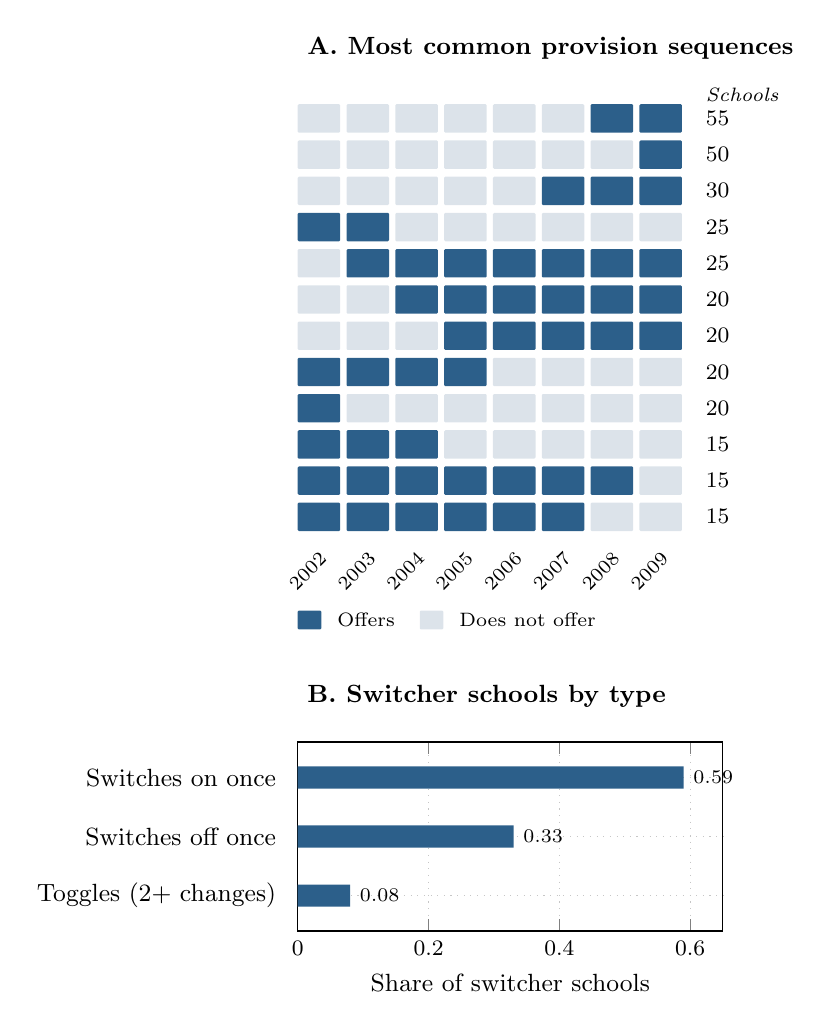
\begin{tikzpicture}

% =====================================================================
% A. Most common provision sequences
% =====================================================================
\begin{scope}[shift={(0,0)}]

\node[anchor=south west, font=\bfseries\small] at (0,0.45)
  {A. Most common provision sequences};

% ---- paste from seq_patterns.txt ----
% cells = one digit per cohort (1 = offers, 0 = does not)
% n     = number of switcher schools with this sequence
\seqrow{1}{0,0,0,0,0,0,1,1}{55}
\seqrow{2}{0,0,0,0,0,0,0,1}{50}
\seqrow{3}{0,0,0,0,0,1,1,1}{30}
\seqrow{4}{1,1,0,0,0,0,0,0}{25}
\seqrow{5}{0,1,1,1,1,1,1,1}{25}
\seqrow{6}{0,0,1,1,1,1,1,1}{20}
\seqrow{7}{0,0,0,1,1,1,1,1}{20}
\seqrow{8}{1,1,1,1,0,0,0,0}{20}
\seqrow{9}{1,0,0,0,0,0,0,0}{20}
\seqrow{10}{1,1,1,0,0,0,0,0}{15}
\seqrow{11}{1,1,1,1,1,1,1,0}{15}
\seqrow{12}{1,1,1,1,1,1,0,0}{15}
% ----------------------------------------

% cohort axis
\foreach \c [count=\i] in {2002,2003,2004,2005,2006,2007,2008,2009} {
  \node[font=\scriptsize, anchor=north, rotate=45, anchor=north east]
    at ({(\i-1)*0.62+0.27}, {-12*0.46+0.02}) {\c};
}
\node[anchor=west, font=\scriptsize\itshape]
  at ({8*0.62+0.10}, {0.12}) {Schools};

% key
\fill[cOffer, rounded corners=0.4pt] (0,{-12*0.46-1.15})
   rectangle +(0.30,0.24);
\node[anchor=west, font=\scriptsize] at (0.38,{-12*0.46-1.03}) {Offers};
\fill[cNoOffer, rounded corners=0.4pt] (1.55,{-12*0.46-1.15})
   rectangle +(0.30,0.24);
\node[anchor=west, font=\scriptsize] at (1.93,{-12*0.46-1.03})
   {Does not offer};

\end{scope}

% =====================================================================
% B. Switcher schools by type of change
% =====================================================================
\begin{axis}[
    name=panelB,
    at={(0cm,-8.1cm)}, anchor=north west,
    scale only axis,
    width=5.4cm, height=2.4cm,
    title={B. Switcher schools by type},
    title style={at={(0,1)}, anchor=south west, yshift=3pt,
                 font=\bfseries\small},
    xbar,
    bar width=8pt,
    xmin=0, xmax=0.65,
    xtick={0,0.2,0.4,0.6},
    xticklabel style={/pgf/number format/fixed, font=\footnotesize},
    xlabel={Share of switcher schools},
    xlabel style={font=\small},
    y dir=reverse,
    symbolic y coords={SwitchOn,SwitchOff,Toggle},
    ytick={SwitchOn,SwitchOff,Toggle},
    yticklabels={{Switches on once},{Switches off once},
                 {Toggles (2+ changes)}},
    yticklabel style={font=\small},
    ytick style={draw=none},
    enlarge y limits=0.30,
    grid=major,
    grid style={dotted, gray!45},
    nodes near coords,
    nodes near coords style={font=\scriptsize,
                             /pgf/number format/fixed,
                             /pgf/number format/precision=2},
]

% ---- paste from seq_types.txt ----
\addplot[fill=cBar, draw=none] coordinates {
    (0.59,SwitchOn)
    (0.33,SwitchOff)
    (0.08,Toggle)
};
% ----------------------------------------

\end{axis}

\end{tikzpicture}}

\label{fig:sequence}
\begin{singlespace}
\fignote{Notes: Restricted to schools whose A-level economics provision
changes at least once across the 2002--2009 GCSE cohorts, and which are
observed in every cohort. Panel A shows the twelve most common provision
sequences, one row per sequence and one cell per cohort; shaded cells
indicate cohorts to which the school offered A-level economics. The
right-hand column gives the number of schools following each sequence.
Sequences followed by fewer than ten schools are suppressed. Panel B
classifies all switcher schools by whether provision changes once or more
than once.}
\end{singlespace}
\end{figure}


% =====================================================================
% Figure: share of schools offering A-level economics over time
% Self-contained apart from: pgfplots, pgfplotstable, compat=1.18
% Numbers pasted from ts_offer.txt
% =====================================================================
\begin{figure}[p]
\caption{Share of schools offering A-level economics over time}
\setlength{\parskip}{0pt}

% ---- styling, local to this figure ----
\definecolor{cLine}{HTML}{2C5F8A}

% ---- paste from ts_offer.txt ----
% year   = GCSE cohort year
% share  = share of schools offering A-level economics
% nsch   = number of schools observed that year
\pgfplotstableread[col sep=space]{
year   share   nsch
2002   0.375   2135
2003   0.372   2135
2004   0.377   2120
2005   0.381   2130
2006   0.396   2135
2007   0.409   2175
2008   0.422   2200
2009   0.448   2665
2010   0.449   2545
2011   0.460   2395
}\tsdata
% ----------------------------------------

\centerline{%
\begin{tikzpicture}
\begin{axis}[
    width=0.72\textwidth,
    height=7.2cm,
    xlabel={GCSE cohort},
    ylabel={Share of schools offering A-level economics},
    xlabel style={font=\small},
    ylabel style={font=\small},
    xtick=data,
    xticklabel style={/pgf/number format/1000 sep={},
                      font=\footnotesize, rotate=45, anchor=north east},
    ymin=0, ymax=0.55,
    ytick={0,0.1,0.2,0.3,0.4,0.5},
    yticklabel style={/pgf/number format/fixed,
                      /pgf/number format/precision=2,
                      font=\footnotesize},
    grid=major,
    grid style={dotted, gray!45},
    enlarge x limits=0.06,
]

\addplot[cLine, thick, mark=*, mark size=2pt]
    table[x=year, y=share] {\tsdata};

\end{axis}
\end{tikzpicture}}

\label{fig:time_series}
\begin{singlespace}
\fignote{Notes: A school is counted as offering A-level economics to a
cohort if at least two students in that school-year group sat the A-level
economics examination. The sample comprises all schools with post-16
provision observed in the given year; the number of schools observed
ranges from around 2,120 to 2,670 per year. Provision is measured in a
wider extract covering GCSE cohorts 2002--2013, so the series extends
beyond the 2002--2008 earnings sample.}
\end{singlespace}
\end{figure}


% =====================================================================
% Figure: event study of A-level economics take-up around provision changes
% Self-contained apart from: pgfplots, pgfplotstable, compat=1.18
% Numbers pasted from es_for_latex.txt
% =====================================================================
\begin{figure}[p]
\caption[Event study: take-up around provision changes]{Event study: A-level economics take-up around provision changes}
\setlength{\parskip}{0pt}

% ---- styling, local to this figure ----
\definecolor{cEvent}{HTML}{2C5F8A}

\pgfplotsset{
  esstyle/.style={
    scale only axis,
    width=6.0cm,
    height=5.2cm,
    xlabel={Cohorts relative to change in provision},
    xlabel style={font=\small},
    xmin=-3.6, xmax=3.6,
    xtick={-3,-2,-1,0,1,2,3},
    xticklabel style={font=\footnotesize},
    yticklabel style={/pgf/number format/fixed,
                      /pgf/number format/precision=2,
                      font=\footnotesize},
    grid=major,
    grid style={dotted, gray!45},
    title style={at={(0.5,1)}, anchor=south, yshift=3pt,
                 font=\bfseries\small},
    ylabel style={font=\small},
    % solid reference line at zero on the y axis
    extra y ticks={0},
    extra y tick style={grid=major, grid style={solid, black!55},
                        tick label style={opacity=0}},
    % dashed line marking the last pre-period
    extra x ticks={-0.5},
    extra x tick style={grid=major,
                        grid style={dashed, black!45},
                        tick label style={opacity=0}},
  },
  esplot/.style={
    cEvent, only marks, mark=*, mark size=1.7pt,
    error bars/.cd, y dir=both, y explicit,
    error bar style={line width=0.6pt, cEvent},
    error mark options={mark size=1.2pt, line width=0.6pt},
  },
}

% ---- paste from es_for_latex.txt ----
% t             = cohorts relative to the change (-1 is the omitted period)
% b_on/lo/hi    = schools that begin offering economics
% b_off/lo/hi   = schools that stop offering economics
\pgfplotstableread[col sep=space]{
t    b_on   lo_on   hi_on   b_off   lo_off  hi_off
-3   0.004  -0.008   0.015   0.012  -0.013   0.037
-2   0.002  -0.005   0.009   0.009  -0.007   0.024
-1   0.000   0.000   0.000   0.000   0.000   0.000
 0   0.014   0.007   0.021  -0.028  -0.044  -0.013
 1   0.071   0.063   0.080  -0.029  -0.049  -0.009
 2   0.072   0.060   0.084  -0.014  -0.040   0.013
 3   0.076   0.060   0.093  -0.005  -0.042   0.032
}\esdata
% ----------------------------------------

\centerline{%
\begin{tikzpicture}

% ============ A. Schools that begin offering ============
\begin{axis}[
    esstyle,
    name=panelA,
    title={A. Schools that begin offering},
    ylabel={Effect on share of cohort taking economics},
    ymin=-0.03, ymax=0.12,
    ytick={-0.02,0,0.02,0.04,0.06,0.08,0.10},
]
\addplot[esplot] table[x=t, y=b_on,
    y error plus expr=\thisrow{hi_on}-\thisrow{b_on},
    y error minus expr=\thisrow{b_on}-\thisrow{lo_on}] {\esdata};
\end{axis}

% ============ B. Schools that stop offering ============
\begin{axis}[
    esstyle,
    name=panelB,
    at={(panelA.south east)}, anchor=south west, xshift=1.35cm,
    title={B. Schools that stop offering},
    ymin=-0.12, ymax=0.03,
    ytick={-0.10,-0.08,-0.06,-0.04,-0.02,0,0.02},
]
\addplot[esplot] table[x=t, y=b_off,
    y error plus expr=\thisrow{hi_off}-\thisrow{b_off},
    y error minus expr=\thisrow{b_off}-\thisrow{lo_off}] {\esdata};
\end{axis}

\end{tikzpicture}}

\label{fig:eventstudy}
\begin{singlespace}
\fignote{Notes: Each point is the coefficient on an indicator for a given cohort before or after the change in A-level economics provision, relative to the cohort just before the change, estimated on switcher schools only. The outcome is the share of
the school-cohort taking A-level economics. Each specification includes
school and cohort fixed effects; the cohort immediately before the change
($t=-1$) is the omitted category, and the dashed line marks the last
pre-change cohort. Bars are 95\% confidence intervals. Panel A covers
schools that begin offering economics, Panel B those that stop; schools
whose provision changes more than once are excluded. Endpoints are binned,
so $t=-3$ and $t=3$ include all earlier and later cohorts respectively.
The number of school-cohorts contributing at each event time is reported
in Appendix Table~\ref{tab:eventstudy_counts}. A test that all the pre-change coefficients are jointly zero gives $p = 0.81$ for Panel A and $p = 0.54$ for Panel B, so there is no evidence that take-up was already changing before provision changed.}
\end{singlespace}
\end{figure}


% =====================================================================
% Figure: event study of cohort KS4 attainment around provision changes
% Self-contained apart from: pgfplots, pgfplotstable, compat=1.18
% Numbers pasted from the KS4 block of es_eventstudy.do (es_ks4.dta)
% Estimated with W = 3
% =====================================================================
\begin{figure}[p]
\caption{Event study: cohort attainment around changes in A-level
economics provision}
\setlength{\parskip}{0pt}

% ---- styling, local to this figure ----
\definecolor{cEvent}{HTML}{2C5F8A}

\pgfplotsset{
  ks4style/.style={
    scale only axis,
    width=6.0cm,
    height=5.4cm,
    xlabel={Cohorts relative to change in provision},
    xlabel style={font=\small},
    xmin=-3.6, xmax=3.6,
    xtick={-3,-2,-1,0,1,2,3},
    xticklabel style={font=\footnotesize},
    ymin=-0.22, ymax=0.22,
    ytick={-0.2,-0.1,0,0.1,0.2},
    yticklabel style={/pgf/number format/fixed,
                      /pgf/number format/precision=1,
                      font=\footnotesize},
    grid=major,
    grid style={dotted, gray!45},
    title style={at={(0.5,1)}, anchor=south, yshift=3pt,
                 font=\bfseries\small},
    ylabel style={font=\small},
    % solid reference line at zero on the y axis
    extra y ticks={0},
    extra y tick style={grid=major, grid style={solid, black!55},
                        tick label style={opacity=0}},
    % dashed line marking the last pre-change cohort
    extra x ticks={-0.5},
    extra x tick style={grid=major,
                        grid style={dashed, black!45},
                        tick label style={opacity=0}},
  },
  ks4plot/.style={
    cEvent, only marks, mark=*, mark size=1.7pt,
    error bars/.cd, y dir=both, y explicit,
    error bar style={line width=0.6pt, cEvent},
    error mark options={mark size=1.2pt, line width=0.6pt},
  },
}

% ---- paste from es_ks4.dta ----
% t             = cohorts relative to the change (-1 is omitted)
% b_on/lo/hi    = schools that begin offering economics
% b_off/lo/hi   = schools that stop offering economics
% Units are standard deviations of the KS4 point score.
\pgfplotstableread[col sep=space]{
t    b_on   lo_on   hi_on   b_off   lo_off  hi_off
-3  -0.003  -0.068   0.062  -0.043  -0.139   0.053
-2  -0.009  -0.033   0.052  -0.017  -0.078   0.044
-1   0.000   0.000   0.000   0.000   0.000   0.000
 0   0.017  -0.024   0.057   0.032  -0.026   0.091
 1   0.029  -0.023   0.082   0.026  -0.051   0.104
 2   0.031  -0.039   0.102   0.052  -0.051   0.154
 3   0.000  -0.098   0.097   0.068  -0.074   0.211
}\ksdata
% ----------------------------------------

\centerline{%
\begin{tikzpicture}

% ============ A. Schools that begin offering ============
\begin{axis}[
    ks4style,
    name=panelA,
    title={A. Schools that begin offering},
    ylabel={Effect on mean KS4 point score (SD)},
]
\addplot[ks4plot] table[x=t, y=b_on,
    y error plus expr=\thisrow{hi_on}-\thisrow{b_on},
    y error minus expr=\thisrow{b_on}-\thisrow{lo_on}] {\ksdata};
\end{axis}

% ============ B. Schools that stop offering ============
\begin{axis}[
    ks4style,
    name=panelB,
    at={(panelA.south east)}, anchor=south west, xshift=1.35cm,
    title={B. Schools that stop offering},
    yticklabels={},
    ylabel={},
]
\addplot[ks4plot] table[x=t, y=b_off,
    y error plus expr=\thisrow{hi_off}-\thisrow{b_off},
    y error minus expr=\thisrow{b_off}-\thisrow{lo_off}] {\ksdata};
\end{axis}

\end{tikzpicture}}

\label{fig:eventstudy_ks4}
\begin{singlespace}
\fignote{Notes: Coefficients on leads and lags of A-level economics
provision, estimated on switcher schools only. The outcome is the mean
standardised KS4 point score of the school-cohort, a characteristic of
the intake determined before any exposure to A-level provision. Each
specification includes school and cohort fixed effects; the cohort
immediately before the change ($t=-1$) is the omitted category, and the
dashed line marks the last pre-change cohort. Bars are 95\% confidence
intervals; both panels share a common vertical scale. Panel A covers
schools that begin offering economics, Panel B those that stop; schools
whose provision changes more than once are excluded. Endpoints are
binned, so $t=-3$ and $t=3$ include all earlier and later cohorts
respectively. The number of school-cohorts contributing at each event time is
reported in Appendix Table~\ref{tab:eventstudy_counts}. A joint test of the pre-change
coefficients gives $p = 0.82$ for Panel A and $p = 0.68$
for Panel B.}
\end{singlespace}
\end{figure}


\FloatBarrier

% =============================================================
% Appendix Tables
% =============================================================

% --- Referenced from Section II ---

% Table: LPM preference vs constraint by subgroup, 2011 cohort (Chapter 4 appendix)
\begin{table}[htbp]
\centering
\caption{Effect of availability and school type on A-level economics take-up by subgroup, 2011 cohort}
\label{tab:lpm_subgroup}
\begin{tabular}{l ccc}
\toprule
                              & $\hat{\beta}$: & Always     & Switcher   \\
                              & effect of  & offer      &            \\
                              & avail.     & vs.\ never & vs.\ never \\
\midrule
All students                  & 0.078\sym{***}& 0.025\sym{***}& 0.0009\sym{***}\\
                              & (0.004)       & (0.005)       & (0.0003)       \\
\addlinespace
Male                          & 0.120\sym{***}& 0.035\sym{***}& 0.0019\sym{***}\\
                              & (0.006)       & (0.007)       & (0.0005)       \\
Female                        & 0.046\sym{***}& 0.012\sym{***}& 0.0003\\
                              & (0.003)       & (0.004)       & (0.0003)       \\
\addlinespace
Non-FSM                       & 0.078\sym{***}& 0.026\sym{***}& 0.0009\sym{***}\\
                              & (0.004)       & (0.005)       & (0.0003)       \\
FSM                           & 0.083\sym{***}& 0.019\sym{**}& 0.0009\\
                              & (0.007)       & (0.009)       & (0.001)       \\
\addlinespace
White British                 & 0.064\sym{***}& 0.021\sym{***}& 0.0004\sym{*}\\
                              & (0.004)       & (0.005)       & (0.0002)       \\
Indian                        & 0.161\sym{***}& 0.045\sym{**}& 0.004\\
                              & (0.017)       & (0.019)       & (0.003)       \\
Pakistani/Bangladeshi         & 0.105\sym{***}& 0.027\sym{**}& 0.0003\\
                              & (0.011)       & (0.014)       & (0.002)       \\
Black African/Caribbean       & 0.122\sym{***}& 0.019& 0.005\\
                              & (0.010)       & (0.012)       & (0.003)       \\
Chinese                       & 0.128\sym{***}& 0.090\sym{***}& 0.006\\
                              & (0.027)       & (0.030)       & (0.011)       \\
\addlinespace
London/South East             & 0.110\sym{***}& 0.014\sym{*}& 0.001\\
                              & (0.006)       & (0.008)       & (0.001)       \\
Rest of England               & 0.060\sym{***}& 0.029\sym{***}& 0.0008\sym{***}\\
                              & (0.003)       & (0.005)       & (0.0003)       \\
\addlinespace
Observations                  & \multicolumn{3}{c}{221,118} \\
\bottomrule
\end{tabular}
\begin{minipage}{\textwidth}
\smallskip
\footnotesize
\textit{Notes:} Each row reports coefficients from a separate LPM of A-level economics take-up on an indicator for availability and school-type dummies (always-offer, switcher; never-offer omitted), estimated on the indicated subgroup from the 2011 GCSE cohort. The availability coefficient $\hat{\beta}$ captures the effect of removing the supply constraint; the school-type coefficients capture preference-side heterogeneity across school environments, holding availability constant. Standard errors clustered at the school level in parentheses. \sym{*} $p<0.10$, \sym{**} $p<0.05$, \sym{***} $p<0.01$.
\end{minipage}
\end{table}


% Table: Access and take-up decomposition, 2003 and 2007 cohorts (Chapter 4 appendix)
\begin{table}[htbp]
\centering
\caption{Access to and take-up of A-level economics by demographic group, 2003 and 2007 cohorts}
\label{tab:pref_constraint_earlier}
\begin{tabular}{l ccccc}
\toprule
                              & Access     & Take-up    & Take-up    & Gap from   & Share of   \\
                              & rate       & $|$ access & (uncondit.)& access     & gap from   \\
                              &            &            &            &            & access     \\
\midrule
\multicolumn{6}{c}{\textbf{2003 cohort}} \\
\midrule
\multicolumn{6}{l}{\textit{Sex}} \\
Male                          & 60.8       & 11.4       & 6.9        &            &            \\
Female                        & 55.7       & 3.6        & 2.0        &            &            \\
Gap (M $-$ F)                 & 5.1        & 7.8        & 4.9        & 0.7        & 14.3       \\
\addlinespace
\multicolumn{6}{l}{\textit{Socioeconomic status}} \\
Non-FSM                       & 58.5       & 7.3        & 4.3        &            &            \\
FSM                           & 55.9       & 6.9        & 3.8 &            &            \\
Gap                           & 2.6        & 0.4        & 0.5        & 0.2        & 40.0       \\
\addlinespace
\multicolumn{6}{l}{\textit{Region}} \\
London/South East             & 67.3       & 8.9        & 6.0        &            &            \\
Rest of England               & 53.3       & 6.3        & 3.4        &            &            \\
Gap                           & 14.0       & 2.6        & 2.6        &  1.1       & 42.3       \\
\addlinespace
\multicolumn{6}{l}{\textit{Ethnicity}} \\
White British                 & 55.6       & 6.2        & 3.5        &            &            \\
Indian                        & 72.4       & 15.4       & 11.1       &            &            \\
Pakistani/Bangladeshi         & 60.1       & 9.2        & 5.6        &            &            \\
Black African/Caribbean       & 69.6       & 9.0        & 6.3        &            &            \\
Chinese                       & 67.2       & 15.3       & 10.3       &            &            \\
\addlinespace
Gap: Indian $-$ White         &            &            & 7.6        & 1.8        & 23.7       \\
Gap: Pak./Bang. $-$ White     &            &            & 2.1        & 0.3        & 14.3       \\
Gap: Black Afr./Car. $-$ White &            &            & 2.8        & 1.1        & 39.3       \\
Gap: Chinese $-$ White        &            &            & 6.8        & 1.2        & 17.6       \\
\addlinespace
$N$                           & \multicolumn{5}{c}{188,957} \\
\bottomrule
\end{tabular}
\end{table}

\clearpage

\begin{table}[htbp]
\ContinuedFloat
\centering
\caption{Access to and take-up of A-level economics by demographic group, 2003 and 2007 cohorts continued}
\label{tab:pref_constraint_earlier_continued}
\begin{tabular}{l ccccc}
\toprule
                              & Access     & Take-up    & Take-up    & Gap from   & Share of   \\
                              & rate       & $|$ access & (uncondit.)& access     & gap from   \\
                              &            &            &            &            & access     \\
\midrule
\multicolumn{6}{c}{\textbf{2007 cohort}} \\
\midrule
\multicolumn{6}{l}{\textit{Sex}} \\
Male                          & 64.6         & 12.6         & 8.2         &            &            \\
Female                        & 59.9         & 8.2         & 2.7         &            &            \\
Gap (M $-$ F)                 & 4.7         & 10.3         & 5.5         & 0.5         & 9.1         \\
\addlinespace
\multicolumn{6}{l}{\textit{Socioeconomic status}} \\
Non-FSM                       & 62.5         & 8.3         & 5.2         &            &            \\
FSM                           & 60.8         & 8.3         & 5.1         &            &            \\
Gap                           & 1.7         & 0.0         & 0.1         & 0.1         & 100.0         \\
\addlinespace
\multicolumn{6}{l}{\textit{Region}} \\
London/South East             & 72.0         & 10.2         & 7.4         &            &            \\
Rest of England               & 56.9         & 7.0         & 4.0         &            &            \\
Gap                           & 15.1         & 3.2         & 3.4         & 1.3         & 38.2         \\
\addlinespace
\multicolumn{6}{l}{\textit{Ethnicity}} \\
White British                 & 59.6         & 6.8         & 4.1         &            &            \\
Indian                        & 73.9         & 18.8         & 14.0         &            &            \\
Pakistani/Bangladeshi         & 63.4         & 12.5         & 8.0         &            &            \\
Black African/Caribbean       & 73.9         & 11.3         & 8.4         &            &            \\
Chinese                       & 72.9         & 17.5         & 12.8         &            &            \\
\addlinespace
Gap: Indian $-$ White         &            &            & 9.9         & 1.8         & 18.2         \\
Gap: Pak./Bang. $-$ White     &            &            & 3.9         & 0.4         & 10.3         \\
Gap: Black Afr./Car. $-$ White &            &            & 4.3         & 1.3         & 30.2         \\
Gap: Chinese $-$ White        &            &            & 8.7         & 1.6         & 18.4         \\
\addlinespace
$N$                           & \multicolumn{5}{c}{211,651} \\
\bottomrule
\end{tabular}

\begin{minipage}{\textwidth}
\smallskip
\footnotesize
\textit{Notes:} Same structure as main-text Table~\ref{tab:access_takeup}, replicated for the 2003 and 2007 GCSE cohorts. Access rate is the share of students attending a school that offers A-level economics (defined as $\geq 2$ students sitting the exam in the school-cohort). Take-up $|$ access is the share taking A-level economics conditional on the school offering it. The ``+ att.'' column additionally controls for standardised GCSE attainment. The take-up gap is decomposed as $p_A - p_B = \bar{c}(a_A - a_B) + \bar{a}(c_A - c_B)$, where $a$ denotes the access rate, $c$ denotes conditional take-up, and bars denote simple averages across the two groups. ``Gap from access'' is the first term; ``Share of gap from access'' divides this by the unconditional take-up gap.
\end{minipage}
\end{table}


% Table: Demographic composition of cohort, university students, and economics UGs (Chapter 4 appendix)
\begin{table}[htbp]
\centering
\caption{Demographic composition of cohort, university students, and economics undergraduates}
\label{tab:composition}
\begin{tabular}{l ccc ccc ccc}
\toprule
                    & \multicolumn{3}{c}{2003}   & \multicolumn{3}{c}{2007}   & \multicolumn{3}{c}{2011}   \\
\cmidrule(l{3pt}r{3pt}){2-4} \cmidrule(l{3pt}r{3pt}){5-7} \cmidrule(l{3pt}r{3pt}){8-10}
                    & Cohort & UGs  & Econ  & Cohort & UGs  & Econ  & Cohort & UGs  & Econ  \\
                    &        &      & UGs   &        &      & UGs   &        &      & UGs   \\
\midrule
\multicolumn{10}{c}{\textbf{Panel A: Sex}} \\
\midrule
Male                & 46.8   & 45.9 & 71.5  & 47.5   & 46.5 & 70.8  & 48.0   & 46.2 & 72.0  \\
Female              & 53.2   & 54.1 & 28.5  & 52.5   & 53.5 & 29.2  & 52.0   & 53.8 & 28.0  \\
\midrule
\multicolumn{10}{c}{\textbf{Panel B: Ethnicity}} \\
\midrule
White British       & 75.3   & 72.5 & 53.6  & 76.2   & 72.6 & 54.2  & 73.0  & 67.7 & 50.1  \\
Black African       & 1.6  & 2.0 & 4.0 & 2.3  & 2.9 & 5.0 & 3.1  & 4.2 & 7.4 \\
Black Caribbean     & 1.2  & 1.4 & 0.9 & 1.3  & 1.5 & 1.0 & 1.4  & 1.6 & 1.5 \\
Indian              & 3.7  & 4.6 & 13.9 & 3.1  & 3.9 & 11.9 & 2.9  & 3.8 & 10.1 \\
Pakistani           & 2.5  & 2.8 & 3.8 & 2.6  & 3.0 & 3.8 & 3.1  & 3.7 & 4.5 \\
Bangladeshi         & 1.0  & 1.1 & 2.1 & 1.1  & 1.2 & 2.7 & 1.4  & 1.7 & 2.4 \\
Chinese             & 0.6  & 0.7 & 2.3 & 0.5  & 0.7 & 2.1 & 0.6  & 0.8 & 2.2 \\
\bottomrule
\end{tabular}
\begin{minipage}{\textwidth}
\smallskip
\footnotesize
\textit{Notes:} Shares of each group in the GCSE cohort, among university students, and among economics undergraduates, for three cohorts. Shares may not sum to one due to omitted categories.
\end{minipage}
\end{table}


% Table: Access to and take-up of A-level economics by school type (Chapter 4 appendix)
\begin{table}[htbp]
\centering
\caption{Access to and take-up of A-level economics by school type}
\label{tab:school_type}
\begin{tabular}{l ccccc}
\toprule
                              & \% offer   & \% offer   & Take-up    & Take-up    & Conversion \\
                              & econ       & maths      & $|$ offer  & $|$ offer  & to econ    \\
                              &            &            & (raw)      & (+ att.)   & degree     \\
\midrule
\multicolumn{6}{c}{\textbf{Panel A: Boys}} \\
\midrule
Mixed                         & 67.8         &    99.1      & 14.1         & XX         & 33.4         \\
Single-sex boys               & 86.9         & 99.5         & 20.0         & XX         & 38.3         \\
\midrule
\multicolumn{6}{c}{\textbf{Panel B: Girls}} \\
\midrule
Mixed                         & 66.4         & 98.6         & 4.8         & XX         & 30.2         \\
Single-sex girls              & 63.1         & 99.3         & 10.6         & XX         & 33.7         \\
\bottomrule
\end{tabular}
\begin{minipage}{\textwidth}
\smallskip
\footnotesize
\textit{Notes:} The table reports the share of schools offering A-level economics and maths, the take-up rate conditional on the school offering economics (raw and controlling for GCSE attainment), and the conversion rate from A-level economics to an economics degree. Sample: 2011 GCSE cohort.
\end{minipage}
\end{table}


% --- Referenced from Section III.A ---

% Table: School characteristics by offer behaviour (Chapter 4 appendix)
\begin{table}[htbp]
\centering
\caption{School characteristics by A-level economics offer behaviour}
\label{tab:school_chars}
\begin{tabular}{l ccc ccc}
\toprule
                              & \multicolumn{3}{c}{2007}               & \multicolumn{3}{c}{2011}               \\
\cmidrule(l{3pt}r{3pt}){2-4} \cmidrule(l{3pt}r{3pt}){5-7}
                              & Always     & Switcher   & Never      & Always     & Switcher   & Never      \\
\midrule
Av.\ KS4 score               & 0.82       & 0.75       & 0.75       & 0.64       & 0.60       & 0.63       \\
\% FSM                        & 5.4        & 6.0        & 5.8        & 5.6        & 7.1        & 7.5       \\
\% White British              & 71         & 76         & 84         & 69         & 73         & 79         \\
\% Black African              & 2.5        & 2.5        & 1.2        & 3.3        & 3.2        & 1.9        \\
\% Indian                     & 4.8        & 3.2        & 2.1        & 4.6        & 2.7        & 2.3        \\
\% Chinese                    & 0.86       & 0.66       & 0.47       & 0.90       & 0.67       & 0.53       \\
\% All boys                   & 8.5        & 4.0        & 2.4        & 8.2        & 2.7        & 2.4        \\
\% All girls                  & 3.9        & 10.9        & 9.5        & 5.7        & 11.3        & 7.4        \\
\addlinespace
N schools                     & 453        & 800      & 924      & 667        & 764        & 966      \\
\bottomrule
\end{tabular}
\begin{minipage}{\textwidth}
\smallskip
\footnotesize
\textit{Notes:} School-level averages by economics offer behaviour. ``Always offer'' schools offer A-level economics in every cohort in our sample; ``Never offer'' schools never offer it; ``Switcher'' schools offer it in some cohorts but not others. Figures correspond to the main-text Figure~\ref{fig:external_validity}.
\end{minipage}
\end{table}


% Table: School transitions at age 16 (Chapter 4 appendix)
\begin{table}[htbp]
\centering
\caption{School transitions at age 16 and A-level economics access}
\label{tab:school_moves}
\begin{tabular}{l cccc}
\toprule
                                          & \multicolumn{4}{c}{KS5 school offer behaviour} \\
\cmidrule(l{3pt}r{3pt}){2-5}
KS4 school offer behaviour                & Always     & Switcher   & Never      & Total      \\
\midrule
\multicolumn{5}{c}{\textbf{Panel A: Transition matrix (\% of KS5 students)}} \\
\midrule
Same school (no move)                     & 17.2         & 20.8         & 17.3         & 55.3         \\
\addlinespace
Moved from: Always offer                  & 2.2        & 0.9         & 0.4         & 3.4         \\
Moved from: Switcher                      & 3.7         & 1.6        & 0.7         & 6.0         \\
Moved from: Never offer                   & 3.4         & 1.8         & 1.0        & 6.2         \\
Moved from: No 6th form and is feeder school                 & 16.4         & 4.0         & 1.4         & 21.9         \\
Moved from: No 6th form and not feeder school                 & 3.4         & 2.5         & 1.4         & 7.3         \\
\addlinespace
Total                                     & 46.2         & 31.6         & 22.2         & 100        \\
\midrule
\multicolumn{5}{c}{\textbf{Panel B: A-level economics take-up among movers (\%)}} \\
\midrule
Moved: non-offer $\rightarrow$ offer      & \multicolumn{4}{c}{6.3}                    \\
Moved: offer $\rightarrow$ non-offer      & \multicolumn{4}{c}{0.2}                    \\
Non-movers at offer schools               & \multicolumn{4}{c}{7.9}                    \\
Non-movers at non-offer schools           & \multicolumn{4}{c}{0.1}                    \\
\addlinespace
Observations                              & \multicolumn{4}{c}{1,409,336}                    \\
\bottomrule
\end{tabular}
\begin{minipage}{\textwidth}
\smallskip
\footnotesize
\textit{Notes:} Panel~A shows the distribution of students across school transition types. ``Same school'' comprises students who remain at the same institution; transfers from feeder schools are shown separately. Offer behaviour (Always, Switcher, Never) is defined over the full sample period, as in Table~\ref{tab:summary_stats}. In Panel~B, offer and non-offer status refer to the school's offer in the relevant cohort year. Panel~B compares A-level economics take-up rates across transition types. Similar take-up rates between movers who gain access and non-movers at offer schools suggest that school moves are not driven by demand for economics. Sample: GCSE cohorts 2002--2008, students continuing to KS5.
\end{minipage}
\end{table}


% Table: Balance tests (Chapter 4 appendix)
\begin{table}[htbp]
\centering
\caption{Balance tests: effect of A-level economics availability on pre-treatment outcomes}
\label{tab:balance}
\begin{tabular}{l cc}
\toprule
                                      & Coefficient    & SE             \\
Dependent variable                    & on availability&                \\
\midrule
Std.\ GCSE overall score             & -0.007             & (0.008)           \\
Std.\ GCSE maths score               & 0.025\sym{***}             & (0.005)          \\
Std.\ KS2 score (age 11)             & 0.001             & (0.004)           \\
\addlinespace
\% female                             & -0.004            & (0.0024)           \\
\% White British                      & -0.008\sym{**}             & (0.004)           \\
\% FSM eligible                       & 0.001             & (0.001)           \\
\% London/South East                  & 0.0004             & (0.0009)           \\
\addlinespace
School FE                             & \multicolumn{2}{c}{\checkmark}  \\
Cohort FE                             & \multicolumn{2}{c}{\checkmark}  \\
Observations                          & \multicolumn{2}{c}{1,335,629--1,409,039}          \\
\bottomrule
\end{tabular}
\begin{minipage}{\textwidth}
\smallskip
\footnotesize
\textit{Notes:} Each row reports the coefficient from a separate regression of the indicated pre-treatment variable on an indicator for A-level economics availability, with school and cohort fixed effects. Small coefficients support the assumption that within-school changes in availability are not driven by shifts in student composition; the two statistically significant rows (GCSE maths and the White British share) are discussed in Section~\ref{sec:framework}, and both variables are controlled directly in the estimating equations. Observations vary by row with the availability of the dependent variable. Standard errors clustered at the school level. Sample: GCSE cohorts 2002--2008, all schools. \sym{*} $p<0.10$, \sym{**} $p<0.05$, \sym{***} $p<0.01$.
\end{minipage}
\end{table}


% Table: Placebo regressions (Chapter 4 appendix)
\begin{table}[htbp]
\centering
\caption{Placebo test: IV estimates for students who do not take A-level economics}
\label{tab:placebo}
\begin{tabular}{l cc}
\toprule
                                      & (1)            & (2)            \\
                                      & Full sample    & Non-A-level    \\
                                      &                & econ students  \\
\midrule
\multicolumn{3}{c}{\textbf{Panel A: Log earnings at age 28}} \\
\midrule
A-level econ available                & 0.008\sym{*}    & -0.002             \\
                                      & (0.004)           & (0.004)           \\
\addlinespace
School FE                             & \checkmark     & \checkmark     \\
Cohort FE                             & \checkmark     & \checkmark     \\
Individual controls                   & \checkmark     & \checkmark     \\
\addlinespace
Observations                          & 368,260             & 357,168             \\
\bottomrule
\end{tabular}
\begin{minipage}{\textwidth}
\smallskip
\footnotesize
\textit{Notes:} Column~(1) reproduces the reduced-form estimates from the full sample for reference. Column~(2) restricts the sample to students who do not take A-level economics. If availability affects earnings for non-takers, this would indicate a direct effect of availability on outcomes, violating the exclusion restriction. Because availability itself moves students out of the non-taker group, the test conditions on a post-treatment choice and is supportive rather than dispositive. Standard errors clustered at the school level in parentheses. Sample: students in switcher schools, GCSE cohorts 2002--2008. \sym{*} $p<0.10$, \sym{**} $p<0.05$, \sym{***} $p<0.01$.
\end{minipage}
\end{table}


% Table: Robustness of earnings estimates (Chapter 4 appendix)
\begin{table}[htbp]
\centering
\caption{Robustness of IV earnings estimates to alternative specifications}
\label{tab:robustness}
\begin{tabular}{l ccc}
\toprule
                                          & First stage  & IV: log      & First-stage \\
                                          & ($\pi_1$)    & earnings     & $F$         \\
\midrule
1. Baseline (linear controls)             & 0.057\sym{***}  & 0.135\sym{*}   & 843 \\
                                          & (0.002)         & (0.069)         &     \\
\addlinespace
2. Saturated, region as London--SE indicator (141 cells) & 0.058\sym{***}  & 0.152\sym{**}  & 891 \\
                                          & (0.002)         & (0.072)         &     \\
\addlinespace
3. School-specific linear trends          & 0.049\sym{***}  & 0.125           & 804 \\
                                          & (0.002)         & (0.097)         &     \\
\addlinespace
4. Region $\times$ year FE                & 0.058\sym{***}  & 0.120\sym{*}   & 760 \\
                                          & (0.002)         & (0.071)         &     \\
\addlinespace
5. Saturated with KS2 attainment          & 0.057\sym{***}  & 0.145\sym{**}  & 823 \\
                                          & (0.002)         & (0.068)         &     \\
\addlinespace
6. Fine saturated (745 cells)             & 0.058\sym{***}  & 0.159\sym{**}  & 890 \\
                                          & (0.002)         & (0.074)         &     \\
\addlinespace
7. DDML                                   & ---             & 0.128\sym{*}   & --- \\
                                          &                 & (0.068)         &     \\
\addlinespace
School FE                                 & \multicolumn{3}{c}{All specifications} \\
Cohort FE                                 & \multicolumn{3}{c}{All specifications} \\
Observations                              & \multicolumn{3}{c}{368,260} \\
\bottomrule
\end{tabular}
\begin{minipage}{\textwidth}
\smallskip
\footnotesize
\textit{Notes:} Each row reports the first-stage coefficient, the IV estimate of the effect of A-level economics on log earnings at age 28, and the first-stage $F$-statistic. Row~1 is the baseline with linear individual controls. Row~2 uses the saturated covariate specification with region entered as a binary London--SE indicator (sex $\times$ ethnicity group $\times$ FSM $\times$ GCSE tercile $\times$ London-SE); the main-text saturated specification instead uses the three-category region (London/South East, rest of England, missing). Row~3 adds school-specific linear time trends. Row~4 replaces cohort FE with region $\times$ year FE. Row~5 replaces GCSE attainment with KS2 (age 11) attainment in the saturated cells. Row~6 uses the fine saturated specification, with GCSE vigintiles in place of terciles. Row~7 uses double/debiased machine learning. Standard errors clustered at the school level in parentheses. Sample: students in switcher schools, GCSE cohorts 2002--2008. The observation count refers to the baseline; the saturated specifications use slightly fewer observations because small cells drop (cf.\ Table~\ref{tab:main} column~4).

\smallskip
\noindent
All first-stage $F$-statistics exceed 104.7, the threshold above which the conventional critical value of 1.96 remains valid under the $tF$ procedure of \citet{lee2022valid}. No adjustment is therefore required in any specification. The $F$-statistics are cluster-robust throughout: with a single instrument, each equals the square of the instrument's cluster-robust $t$-statistic.

\smallskip
\noindent
Row~7 reports no first-stage coefficient or $F$-statistic because DDML does not estimate a first stage in the two-stage least squares sense. Following \citet{chernozhukov2018dml}, the conditional expectations of the treatment and the instrument given the covariates are estimated by lasso with cross-fitting, and the treatment effect is recovered from the resulting orthogonalised moment condition. There is accordingly no single coefficient on availability to report, and conventional weak-instrument diagnostics do not apply. For reference, the linear first stage estimated on the same sample is reported in row~1.

\smallskip
\noindent
\sym{*} $p<0.10$, \sym{**} $p<0.05$, \sym{***} $p<0.01$.
\end{minipage}
\end{table}


% --- Referenced from Section III.D--E ---

% Table: Effect of A-level economics availability on other educational outcomes (Chapter 4 appendix)
\begin{table}[htbp]
\centering
\caption{Effect of A-level economics availability on other educational outcomes}
\label{tab:other_outcomes}
\begin{tabular}{l cc}
\toprule
                                      & Reduced form   & IV             \\
                                      & (availability) & (A-level econ) \\
\midrule
Attends university                    & 0.008\sym{***}             & 0.140\sym{***}             \\
                                      & (0.002)           & (0.040)           \\
\addlinespace
Attends Russell Group university      & 0.003             & 0.061             \\
                                      & (0.002)           & (0.043)           \\
\addlinespace
Studies economics at UG               & 0.009\sym{***}    & 0.152\sym{***}    \\
                                      & (0.001)           & (0.010)           \\
\addlinespace
Studies business/finance/management   & 0.002             & 0.040             \\
                                      & (0.0014)           & (0.025)           \\
\addlinespace
Studies other STEM                    & -0.003             & -0.044             \\
                                      & (0.002)           & (0.040)           \\
\addlinespace
Studies humanities/social science     & 0.002             & 0.034             \\
                                      & (0.002)           & (0.028)           \\
\addlinespace
Completes degree                      & 0.006\sym{**}             & 0.110\sym{**}             \\
                                      & (0.003)           & (0.050)           \\
\addlinespace
School FE                             & \checkmark     & \checkmark     \\
Cohort FE                             & \checkmark     & \checkmark     \\
Individual controls                   & \checkmark     & \checkmark     \\
\addlinespace
Observations                          & 417,845             & 417,849             \\
\bottomrule
\end{tabular}
\begin{minipage}{\textwidth}
\smallskip
\footnotesize
\textit{Notes:} Each row reports the coefficient from a separate regression. Column~(1) is the reduced form: effect of school-cohort A-level economics availability on the indicated outcome. Column~(2) instruments A-level economics take-up with availability (linear controls specification). The economics UG row repeats the main-text estimate for comparison. Standard errors clustered at the school level in parentheses. Sample: students in switcher schools, GCSE cohorts 2002--2008. \sym{*} $p<0.10$, \sym{**} $p<0.05$, \sym{***} $p<0.01$.
\end{minipage}
\end{table}


% Table: A-level subject combinations by economics availability (Chapter 4 appendix)
\begin{table}[htbp]
\centering
\caption{A-level subject combinations by economics availability}
\label{tab:subject_triples}
\begin{tabular}{l cc cc}
\toprule
                                  & \multicolumn{2}{c}{Switcher schools}  & Always     & Never      \\
\cmidrule(l{3pt}r{3pt}){2-3}
                                  & Econ        & Econ not    & offer      & offer      \\
                                  & available   & available   &            &            \\
\midrule
\multicolumn{5}{c}{\textbf{Panel A: Most common subject triples (\% of students)}} \\
\midrule
Maths, Economics, Physics         & 0.32          & ---         & 0.46         & ---        \\
Maths, Business, Physics          & 0.20          & 0.25          & 0.17         & 0.23         \\
Maths, Biology, Chemistry          & 3.29          & 3.08          & 3.86         & 2.91         \\
Maths, Geography, Physics         & 0.34          & 0.46          & 0.34         & 0.40         \\
Maths, History, Physics           & 0.21          & 0.21          & 0.17         & 0.21         \\
Sciences triple                   & 0.94          & 0.88          & 0.73         & 1.01         \\
Humanities triple                 & 10.2          & 11.2          & 8.4         & 11.1         \\
Other combinations                & 84.5          & 84.0          & 85.9         & 84.1       \\
\midrule
\multicolumn{5}{c}{\textbf{Panel B: Compliers' counterfactual subject bundle (\%)}} \\
\midrule
Business/management               & \multicolumn{2}{c}{24.7}                &            &            \\
Mathematics                       & \multicolumn{2}{c}{-7.7}                &            &            \\
Geography                         & \multicolumn{2}{c}{1.5}                &            &            \\
History                           & \multicolumn{2}{c}{8.0}                &            &            \\
Sciences                          & \multicolumn{2}{c}{-1.8}                &            &            \\
English literature                          & \multicolumn{2}{c}{23.3}                &            &            \\
Psychology                          & \multicolumn{2}{c}{7.0}                &            &            \\
\addlinespace
Observations                      & 104,374          & 117,200          & 321,263         & 138,754         \\
\bottomrule
\end{tabular}
\begin{minipage}{\textwidth}
\smallskip
\footnotesize
\textit{Notes:} Panel~A compares the distribution of A-level subject triples across school-cohorts in switcher schools when economics is and is not available, and in always-offer and never-offer schools. Panel~B reports the composition of the subjects compliers would have taken instead of economics. Each subject's take-up indicator is regressed on economics availability within switcher schools, with school and cohort fixed effects; every student in this sample takes exactly three A-levels, so each student who takes up economics drops exactly one other subject. The entry is the fall in that subject's take-up divided by the rise in economics take-up, expressed as a percentage. It is the share of compliers who would otherwise have taken that subject. Shares sum to 100 across all subjects; those shown account for 55\%, with the remainder spread across smaller subjects. A negative entry means the subject is taken more, not less, when economics is available: mathematics and the sciences are complements to economics rather than substitutes. The counterfactual mix in Section~\ref{sec:lifetime} is weighted by the positive entries. Sample: GCSE cohorts 2002--2008, students taking exactly three A-levels.
\end{minipage}
\end{table}


% Table: IV estimates by predicted propensity to take A-level economics (Chapter 4 appendix)
\begin{table}[htbp]
\centering
\caption{IV estimates by predicted propensity to take A-level economics}
\label{tab:propensity_heterogeneity}
\begin{tabular}{l cccc}
\toprule
                              & (1)        & (2)        & (3)        & (4)        \\
                              & Bottom     & Second     & Third      & Top        \\
                              & quartile   & quartile   & quartile   & quartile   \\
\midrule
\multicolumn{5}{c}{\textbf{Panel A: First stage (availability $\rightarrow$ A-level econ)}} \\
\midrule
A-level econ available        & XX\sym{***}& XX\sym{***}& XX\sym{***}& XX\sym{***}\\
                              & (XX)       & (XX)       & (XX)       & (XX)       \\
\addlinespace
$F$                           & XX         & XX         & XX         & XX         \\
\midrule
\multicolumn{5}{c}{\textbf{Panel B: IV estimate (A-level econ $\rightarrow$ log earnings)}} \\
\midrule
Takes A-level economics       & XX         & XX         & XX         & XX         \\
                              & (XX)       & (XX)       & (XX)       & (XX)       \\
\addlinespace
School FE                     & \checkmark & \checkmark & \checkmark & \checkmark \\
Cohort FE                     & \checkmark & \checkmark & \checkmark & \checkmark \\
Individual controls           & \checkmark & \checkmark & \checkmark & \checkmark \\
\addlinespace
Observations                  & XX         & XX         & XX         & XX         \\
\bottomrule
\end{tabular}
\begin{minipage}{\textwidth}
\smallskip
\footnotesize
\textit{Notes:} The sample is divided into quartiles of the predicted propensity to take A-level economics, estimated from pre-treatment characteristics (GCSE attainment, sex, ethnicity, FSM status, region, and school-level covariates) using a probit model. Propensity scores are constructed exclusively from variables determined before the availability shock. The IV specification instruments A-level economics take-up with school-cohort availability (linear controls). Standard errors clustered at the school level in parentheses. Sample: GCSE cohorts 2002--2009. \sym{*} $p<0.10$, \sym{**} $p<0.05$, \sym{***} $p<0.01$.
\end{minipage}
\end{table}


% Table: Sensitivity to the availability threshold (Chapter 4 appendix)
\begin{table}[htbp]
\centering
\caption{Sensitivity of the main results to the availability threshold}
\label{tab:threshold_robustness}
\begin{tabular}{l ccc}
\toprule
Threshold (students sitting exam)  & First stage & First-stage $F$ & IV estimate \\
\midrule
$\geq 1$                           & 0.049       & 785             & 0.162       \\
                                   & (0.0018)    &                 & (0.077)     \\
\addlinespace
$\geq 2$ (baseline)                & 0.057       & 843             & 0.135       \\
                                   & (0.0020)    &                 & (0.070)     \\
\addlinespace
$\geq 3$                           & 0.060       & 806             & 0.172       \\
                                   & (0.0021)    &                 & (0.069)     \\
\addlinespace
$\geq 4$                           & 0.060       & 740             & 0.216       \\
                                   & (0.0022)    &                 & (0.064)     \\
\addlinespace
$\geq 5$                           & 0.061       & 737             & 0.256       \\
                                   & (0.0022)    &                 & (0.064)     \\
\bottomrule
\end{tabular}
\begin{minipage}{\textwidth}
\smallskip
\footnotesize
\textit{Notes:} Each row re-estimates the first-stage and IV specifications of Table~\ref{tab:main} under an alternative definition of availability: a school-cohort is coded as offering A-level economics if at least the stated number of students sit the A-level economics exam. The baseline definition in the main text requires two students, and that row reproduces Table~\ref{tab:main}. Standard errors in parentheses. For thresholds other than two, the first-stage $F$ is implied by the ratio of the coefficient to its standard error, computed before rounding. The estimate rises with stricter thresholds, consistent with stricter definitions selecting better-established provision. The sample is that of Table~\ref{tab:main}. The IV estimate is smallest at the baseline threshold, so the baseline definition is conservative.
\end{minipage}
\end{table}


% Table: School-cohorts contributing at each event time (Chapter 4 appendix)
\begin{table}[htbp]
\centering
\caption{School-cohorts contributing at each event time}
\label{tab:eventstudy_counts}
\begin{tabular}{c cc}
\toprule
Event time & Begin offering & Stop offering \\
\midrule
$-3$       & 445            & 175           \\
$-2$       & 190            & 100           \\
$-1$       & 215            & 125           \\
$0$        & 215            & 125           \\
$1$        & 165            & 105           \\
$2$        & 110            & 90            \\
$3$        & 135            & 130           \\
\bottomrule
\end{tabular}
\begin{minipage}{\textwidth}
\smallskip
\footnotesize
\textit{Notes:} The table reports the number of school-cohort observations contributing to each event-time coefficient in Figures~\ref{fig:eventstudy} and~\ref{fig:eventstudy_ks4}. The sample comprises switcher schools observed without gaps whose provision changes exactly once. Endpoints are binned, so $t=-3$ and $t=3$ include all earlier and later cohorts respectively, and a school can contribute more than one cohort to these cells; at interior event times each school contributes one cohort. Counts are rounded to the nearest five in line with the disclosure rules of the secure research environment.
\end{minipage}
\end{table}

